% The document class supplies options to control rendering of some standard
% features in the result.  The goal is for uniform style, so some attention 
% to detail is *vital* with all fields.  Each field (i.e., text inside the
% curly braces below, so the MEng text inside {MEng} for instance) should 
% take into account the following:
%
% - author name       should be formatted as "FirstName LastName"
%   (not "Initial LastName" for example),
% - supervisor name   should be formatted as "Title FirstName LastName"
%   (where Title is "Dr." or "Prof." for example),
% - degree programme  should be "BSc", "MEng", "MSci", "MSc" or "PhD",
% - dissertation title should be correctly capitalised (plus you can have
%   an optional sub-title if appropriate, or leave this field blank),
% - dissertation type should be formatted as one of the following:
%   * for the MEng degree programme either "enterprise" or "research" to
%     reflect the stream,
%   * for the MSc  degree programme "$X/Y/Z$" for a project deemed to be
%     X%, Y% and Z% of type I, II and III.
% - year              should be formatted as a 4-digit year of submission
%   (so 2014 rather than the academic year, say 2013/14 say).

\documentclass[ oneside,tikz,% the name of the author
                    author={Joshua Felmeden},
                % the degree programme: BSc, MEng, MSci or MSc.
                    degree={MEng},
                % the dissertation    title (which cannot be blank)
                     title={Semantic Analysis of Financial Headlines Based on Realised Stock Returns},
                % the dissertation subtitle (which can    be blank)
                  subtitle={Research}]{dissertation}

\usepackage{tabularx}
\usepackage{booktabs}
\usepackage{multirow}
\usepackage{pgfplots}
\usepackage{pgfplotstable}
\usepackage{siunitx}
\usepackage{graphicx}

\edef\restoreparindent{\parindent=\the\parindent\relax}
\usepackage{parskip}
\restoreparindent
% \setlength{\parskip}{\baselineskip}%
\AtBeginDocument{\addtocontents{toc}{\protect\setlength{\parskip}{0pt}}}
\makeatletter
\patchcmd{\@chapter}
  {\addtocontents{lof}}
  {\addtocontents{loa}{\protect\addvspace{10pt}}\addtocontents{lof}}
  {}{}
\makeatother
\usepackage{titlesec}

% \titlespacing*\chapter{0pt}{12pt plus 4pt minus 2pt}{0pt plus 2pt minus 2pt}
% \titlespacing*\section{0pt}{12pt plus 4pt minus 2pt}{0pt plus 2pt minus 2pt}
% \titlespacing*\subsection{0pt}{12pt plus 4pt minus 2pt}{0pt plus 2pt minus 2pt}
% \titlespacing*\subsubsection{0pt}{12pt plus 4pt minus 2pt}{0pt plus 2pt minus 2pt}
\pgfplotsset{compat=1.12}
\usetikzlibrary{
    pgfplots.dateplot,
}
\usepackage{subcaption}
\newcommand\setrow[1]{\gdef\rowmac{#1}#1\ignorespaces}
\newcommand\clearrow{\global\let\rowmac\relax}
\clearrow

\begin{document}

% =============================================================================

% This section simply introduces the structural guidelines.  It can clearly
% be deleted (or commented out) if you use the file as a template for your
% own dissertation: everything following it is in the correct order to use 
% as is.

% \section*{Prelude}
% \thispagestyle{empty}

% A typical dissertation will be structured according to (somewhat) standard 
% sections, described in what follows.  However, it is hard and perhaps even 
% counter-productive to generalise: the goal is {\em not} to be prescriptive, 
% but simply to act as a guideline.  In particular, each page count given is
% important but {\em not} absolute: their aim is simply to highlight that a 
% clear, concise description is better than a rambling alternative that makes
% it hard to separate important content and facts from trivia.

% % You can use this document as a \LaTeX-based~\cite{latexbook1,latexbook2} 
% template for your own dissertation by simply deleting extraneous sections
% and content; keep in mind that the associated {\tt Makefile} could be of
% use. %, in particular because it automatically executes \mbox{\BibTeX} to 
% deal with the associated bibliography. 
% Alternatively, upload this template, dissertation.bib, dissertation.cls, 
% dtklogos.sty and the "logo" folder to Overleaf (an online \LaTeX editor and compiler) and work on your thesis there.

% \textbf{Do not include this section in your final dissertation --- just delete it from the source.}

% =============================================================================

% This macro creates the standard UoB title page by using information drawn
% from the document class (meaning it is vital you select the correct degree 
% title and so on).

\maketitle

% After the title page (which is a special case in that it is not numbered)
% comes the front matter or preliminaries; this macro signals the start of
% such content, meaning the pages are numbered with Roman numerals.

\frontmatter


%\lstlistoflistings

% The following sections are part of the front matter, but are not generated
% automatically by LaTeX; the use of \chapter* means they are not numbered.

% -----------------------------------------------------------------------------

\chapter*{Abstract}

{\bf A compulsory section, of at most 300 words} 
\vspace{1cm} 

\noindent
This section should pr\'{e}cis the project context, aims and objectives,
and main contributions (e.g., deliverables) and achievements; the same 
section may be called an abstract elsewhere.  The goal is to ensure the 
reader is clear about what the topic is, what you have done within this 
topic, {\em and} what your view of the outcome is.

The former aspects should be guided by your specification: essentially 
this section is a (very) short version of what is typically the first 
chapter. If your project is experimental in nature, this should include 
a clear research hypothesis.  This will obviously differ significantly
for each project, but an example might be as follows:

\begin{quote}
My research hypothesis is that a suitable genetic algorithm will yield
more accurate results (when applied to the standard ACME data set) than 
the algorithm proposed by Jones and Smith, while also executing in less
time.
\end{quote}

\noindent
The latter aspects should (ideally) be presented as a concise, factual 
bullet point list.  Again the points will differ for each project, but 
an might be as follows:

\begin{quote}
\noindent
\begin{itemize}
\item I spent $120$ hours collecting material on and learning about the 
      Java garbage-collection sub-system. 
\item I wrote a total of $5000$ lines of source code, comprising a Linux 
      device driver for a robot (in C) and a GUI (in Java) that is 
      used to control it.
\item I designed a new algorithm for computing the non-linear mapping 
      from A-space to B-space using a genetic algorithm, see page $17$.
\item I implemented a version of the algorithm proposed by Jones and 
      Smith in [6], see page $12$, corrected a mistake in it, and 
      compared the results with several alternatives.
\end{itemize}
\end{quote}

% -----------------------------------------------------------------------------


\chapter*{Dedication and Acknowledgements}

% {\bf A compulsory section}
% \vspace{1cm} 

% \noindent
% It is common practice (although totally optional) to acknowledge any
% third-party advice, contribution or influence you have found useful
% during your work.   include support from friends or family, 
% the input of your Supervisor and/or Advisor, external organisations 
% or persons who  have supplied resources of some kind (e.g., funding, 
% advice or time), and so on.

I am very fortunate to work with my superviser Rami Chehab, who assisted in my research greatly and inspired the vast quantity of this project. He has been a great mentor.

I would also like to thank my friends and family for always being there for me, especially when the going gets rough. You guys really helped make this university experience what it was.


% -----------------------------------------------------------------------------


% \chapter*{COVID-19 Statement}

% {\bf An optional section, of at most 800 words} 
% \vspace{1cm} 

% \noindent
% A summary of any planned research activities disrupted by Covid-19 restrictions and the extent to which it was possible to adapt the work in those changed circumstances. If the project was able to go forward as planned, you can safely remove this section without losing any marks. The following may be included:

% \begin{itemize}
% \item Details of any planned research activities curtailed by the pandemic because of, for example, lack of access to facilities, libraries, archives, research participants, fieldwork, etc. Information on any curtailed training should be included only insofar as it relates to the impact on research activities and on the dissertation.

% \item An acknowledgement of the anticipated contribution and value to the dissertation if those research activities had not been curtailed and what was possible to include in the dissertation in the circumstances, including where alternative choices were made to adapt the work and whether there are any weaknesses that could not be overcome.

% \item Any other relevant factors on the impact of Covid-19 on research activities and on the contents of the dissertation.

% \item Details of any research activities required by the examiners as part of a resubmission that were curtailed by the pandemic may be included in a new or revised Covid-19 statement in the resubmitted dissertation.
% \end{itemize}

% -----------------------------------------------------------------------------

% This macro creates the standard UoB declaration; on the printed hard-copy,
% this must be physically signed by the author in the space indicated.

\makedecl



% -----------------------------------------------------------------------------

% LaTeX automatically generates a table of contents, plus associated lists 
% of figures and tables.  These are all compulsory parts of the dissertation.

\tableofcontents
\listoffigures
\listoftables

% -----------------------------------------------------------------------------



\chapter*{Ethics Statement}

{\bf A compulsory section} 
\vspace{1cm} 

In almost every project, this will be one of the following statements:
    \begin{itemize}
        \item ``This project did not require ethical review, as determined by my supervisor, [fill in name]''; or
        \item ``This project fits within the scope of ethics application 0026, as reviewed by my supervisor, [fill in name]''; or
        \item ``An ethics application for this project was reviewed and approved by the faculty research ethics committee as application [fill in number]''.
    \end{itemize}
    
See Section 3.2 of the unit Handbook for more information. If something went wrong and none of those three statements apply, then you should instead explain what happened.


% -----------------------------------------------------------------------------

% \chapter*{Summary of Changes}

% {\bf A conditional section} 
% \vspace{1cm} 

% If and only if the dissertation represents a resubmission (e.g., as the result of
% a resit), this section is compulsory: the content should summarise all
% non-trivial changes made to the initial submission.  Otherwise you can
% omit it, since a summary of this type is clearly nonsensical.

% When included, the section will ideally be used to highlight additional
% work completed, and address criticism raised in any associated feedback.
% Clearly it is difficult to give generic advice about how to do so, but
% an example might be as follows:

% \begin{quote}
% \noindent
% \begin{itemize}
% \item Feedback from the initial submission criticised the design and 
%       implementation of my genetic algorithm, stating ``there seems 
%       to have been no attention to computational complexity during the
%       design, and obvious methods of optimisation are missing within
%       the resulting implementation''.  Chapter $3$ now includes a
%       comprehensive analysis of the algorithm, in terms of both time
%       and space.  While I have not altered the algorithm itself, I
%       have included a cache mechanism (also detailed in Chapter $3$)
%       that provides a significant improvement in average run-time.
% \item I added a feature in my implementation to allow automatic rather
%       than manual selection of various parameters; the experimental
%       results in Chapter $4$ have been updated to reflect this.
% \item Questions after the presentation highlighted a range of related
%       work that I had not considered: I have make a number of updates 
%       to Chapter $2$, resolving this issue.
% \end{itemize}
% \end{quote}

% -----------------------------------------------------------------------------

\chapter*{Supporting Technologies}

% {\bf An optional section}
% \vspace{1cm} 

% \noindent
% This section should present a detailed summary, in bullet point form, 
% of any third-party resources (e.g., hardware and software components) 
% used during the project.  Use of such resources is always perfectly 
% acceptable: the goal of this section is simply to be clear about how
% and where they are used, so that a clear assessment of your work can
% result.  The content can focus on the project topic itself (rather,
% for example, than including ``I used \mbox{\LaTeX} to prepare my 
% dissertation''); an example is as follows:

% \begin{quote}
% \noindent
% \begin{itemize}
% \item I used the Java {\tt BigInteger} class to support my implementation 
%       of RSA.
% \item I used a parts of the OpenCV computer vision library to capture 
%       images from a camera, and for various standard operations (e.g., 
%       threshold, edge detection).
% \item I used an FPGA device supplied by the Department, and altered it 
%       to support an open-source UART core obtained from 
%       \url{http://opencores.org/}.
% \item The web-interface component of my system was implemented by 
%       extending the open-source WordPress software available from
%       \url{http://wordpress.org/}.
% \end{itemize}
% \end{quote}

\begin{itemize}
      \item I used a sample of headlines from Kaggle as training and validation data (\url{https://www.kaggle.com/datasets/miguelaenlle/massive-stock-news-analysis-db-for-nlpbacktests})
      \item I used the Natural Language Toolkit to assist the preprocessing of data, using their English words and stop words data (\url{https://www.nltk.org/})
\end{itemize}


% -----------------------------------------------------------------------------

\chapter*{Notation and Acronyms}

\begin{quote}
\noindent
\begin{tabular}{lcl}
NLP               &:    &     Natural Language Processing \\
SESTM             &:    &     Semantic Extraction via Screening and Topic Modelling \\
\\
\textbf{SESTM Specific Notation} \\
$m$               &:    &     Number of words in sample \\
$n$               &:    &     Number of articles in sample \\
$d_{i,j}$         &:    &     Number of times word $j$ appears in text $i$ \\
$d_{[S],i}$       &:    &     Subset of columns where the only indices are those with sentiment \\
$D = [d_1, \dots, d_n]$ &:    & $m \times n$ Document term matrix \\
$sgn(y)$          &:    &     Sign of returns of article y \\
$\hat x$          &:    &    Expected value of variable $x$ \\
\end{tabular}
\end{quote}


% =============================================================================

% After the front matter comes a number of chapters; under each chapter,
% sections, subsections and even subsubsections are permissible.  The
% pages in this part are numbered with Arabic numerals.  Note that:
%
% - A reference point can be marked using \label{XXX}, and then later
%   referred to via \ref{XXX}; for example Chapter\ref{chap:context}.
% - The chapters are presented here in one file; this can become hard
%   to manage.  An alternative is to save the content in seprate files
%   the use \input{XXX} to import it, which acts like the #include
%   directive in C.

\mainmatter



\chapter{Introduction}
\label{chap:context}
\section{Motivation}
\label{sec:motivation}
Financial news is a widely available resource that offers crucial information on the health and status of the stock market and operating businesses. A huge volume of content is created each day, to such an extent that it is virtually impossible for manual methods to keep up with, leading to developments in automated analysis. With the growth of natural language processing techniques, it has become possible to observe a news article and extract the sentiment of an article; exploiting this information as an indicator of potential future movement of the stock market.

An article is naturally formed of two parts, the headline and the article body. The headline itself is a unique text type, in that it is often not written by the author of the article, and serves as an attractor to a reader that encapsulates the story as a whole \cite{language-newspapers}. In attempting to fulfil this role, headlines have come to have a vocabulary that is alien from other vocabularies, and can sometimes be ambiguous or misleading in the attempt to draw a reader in to read the full article. The words chosen to be included in the headline therefore carry significant meaning, since they intend to convey a lot of information with far fewer words than other text types.

When analysing the sentiment of an article, the body is usually used as input, since the bulk of the information conveyed by a given article is in the body. However, since headlines are a summarisation of the body, it is possible to mine information from the headline itself with as much success as the information collected from the body \cite{headline-sentiment}. The lower word counts of headlines mean processing the data is much quicker, as well as being easier to collect large quantites of headlines.

With financial news outlets portraying the state of markets in such detail, the relationship between the words used in a news article and the effect on the stock market is one that can be utilised to predict future retunrs. In 2019, Ke et Al. \cite{sestm} proposed a novel text mining algorithm that observed previous articles, and their subsequent effect on associated firm share prices, and reteroactively assigned sentiment to words in each article, creating a probabilistic model that can be used to effectively predict future movement of stocks based on news articles on a given day. They state that the algorithm could be extended to use any text based data with some teaching signal, in their case news articles as the text data, and the realised return of the associated stock. Analysing headlines in a similar manner would be beneficial as the headline of an article are both more readily available and shorter, meaning shorter computation times.

\newpage

\section{Aims and Objectives}
The aims and objectives for this project are the following:
\begin{enumerate}
\item Implement and optimise the algorithm proposed by \cite{sestm}
\item Train a model based using a dataset of financial news headlines, with the associated stock returns as a teaching signal.
\item Evaluate the predictive success of the trained model by creating portfolios according to predicted sentiment
\item Compare the performance of the algorithm against other sentiment analysis techniques
\end{enumerate}

% \section{What to do}

% \noindent
% This chapter should introduce the project context and motivate each of the proposed aims and objectives.  Ideally, it is written at a fairly high-level, and easily understood by a reader who is technically competent but not an expert in the topic itself.

% In short, the goal is to answer three questions for the reader.  First, what is the project topic, or problem being investigated?  Second, why is the topic important, or rather why should the reader care about it?  For example, why there is a need for this project (e.g., lack of similar software or deficiency in existing software), who will benefit from the project and in what way (e.g., end-users, or software developers) what work does the project build on and why is the selected approach either important and/or interesting (e.g., fills a gap in literature, applies results from another field to a new problem).  Finally, what are the central challenges involved and why are they significant? 
 
% The chapter should conclude with a concise bullet point list that summarises the aims and objectives.  For example:

% \begin{quote}
% \noindent
% The high-level objective of this project is to reduce the performance 
% gap between hardware and software implementations of modular arithmetic.  
% More specifically, the concrete aims are:

% \begin{enumerate}
% \item Research and survey literature on public-key cryptography and
%       identify the state of the art in exponentiation algorithms.
% \item Improve the state of the art algorithm so that it can be used
%       in an effective and flexible way on constrained devices.
% \item Implement a framework for describing exponentiation algorithms
%       and populate it with suitable examples from the literature on 
%       an ARM7 platform.
% \item Use the framework to perform a study of algorithm performance
%       in terms of time and space, and show the proposed improvements
%       are worthwhile.
% \end{enumerate}
% \end{quote}

% -----------------------------------------------------------------------------

\chapter{Background}
\label{chap:technical}

I begin by discussing the technical background that relates to the work in the dissertation, to provide a foundation from which to build the rest of the project.

\section{Sentiment Analysis}
Sentiment analysis (also known as opinion mining) is the task of identifying opinions or sentiment of authors from an input of text. The implications of being able to programmatically extract the intended meaning of an input are profound and its application could prove valuable in a variety of fields, especially in a financial context. The nuances of natural language can sometimes make this difficult to extract, and therefore significant research has been conducted on the topic throughout previous decades.

The success or failure of any approach to this task can be summarised as the closeness of a prediction of sentiment to that calculated by a human. Take, for example, the following sentences:

\begin{enumerate}
\item \textit{`The movie was great'}
\item \textit{`The movie was terrible'}
\item \textit{`The acting was terrible, but the movie was great'}
\end{enumerate}

Sentences 1 and 2 have very simple sentiment: one is positive, and the other is negative. However, sentence 3 has slightly more complex sentiment. If the feature of interest is the movie, the word \textit{`terrible'} does not influence the sentiment of this feature as it is used in reference to the acting. Simpler analysis methods may not pick up on such nuances in language.

\subsection{Pre processing}
Here, I introduce three terms used in the pre-processing of text data. The main goal of pre-processing in sentiment analysis is to ensure sentiment is being assigned to the correct words. Stop words are a term used in NLP to describe very commonly used words that are considered unimportant (such as `and' or `the'). They serve only as noise and are removed to focus on more impactful words. 

Stemming and lemmatisation are two techniques whose primary is to reduce different forms of a word to its common base form. For example, `am, are, is' all become `be' as it is the root of the word \parencite{stem-lem}. The two techniques share a common goal, but achieve this in different ways. Stemming refers to a more crude process that is effective at the potential cost of precision. In general, it consists of applying a series of rules sequentially, each of which reducing a word. For each reduction, there are conventions to select certain rules. There are a variety of stemmers that each perform stemming in a unique way. On the other hand, lemmatisers are a tool from NLP that does analysis to identify the \textit{lemma}, or the language word root. Both techniques have advantages and disadvantages and as a result the two are often used in tandem, as they compliment one another.

The textual input to any sentiment analysis algorithm requires high quality preprocessing to ensure that the data is of the same format, and is one of the primary steps in any technique. Keeping noisy features such as stop words, or HTML tags serves to muddy the output. Instead, only features of interest should be considered in the ideal scenario \parencite{haddi2013preprocessing}. Insufficient data pre-processing can lead to underachieving analysis models, and as such the importance of this step should not be overlooked. Traditionally, this consists of online text cleaning (if necessary), removal of stop words and whitespace, and stemming and lemmatisation.

\subsection{Lexicon Based Methods}
The fundamental concept of sentiment analysis revolves around investigating a piece of text and deciding on a binary classification: positive or negative. The simplest method involves compiling a weighted word list, known as a lexicon. The weight of a word corresponds to the associated positivity or negativity of the word (for example `great' would have a high positivity, while `terrible' would have a very high negativity score) \parencite{taboada2011lexicon}. The overall sentiment of a piece of text could then be estimated by summing the individual positive sentiment scores of each word while subtracting the negative sentiment scores to yield an overall score for a piece of text. This lexicon is not limited to single words, and can be expanded to include $n$-grams (phrases of $n$ words), as the context in which a word is used can dramatically change its sentiment. This may increase the accuracy of the dictionary at the cost of increased dimensionality. The lexicon itself must be compiled before it is possible to utilise this method, and is normally constructed via in-depth analysis of many texts. An example of a lexicon used for English text is the Harvard-IV-4 psychosociological lexicon (H4) which is a general usage model that can be used to estimate the sentiment of a piece of text.

Certain words that may have no meaning at all in one context, may have significant sentiment in another, particularly in the field of finance, where jargon dominates text. \textcite{lm-dict} conducted an investigation into the use of standard lexicons for analysing 10-K filing reports, which are comprehensive reports filed by companies about their financial performance. They discovered that almost 75\% of negative words found in the filings based on the H4N file were not typically negative in a financial context. For example, `liability' is a negatively charged word in a standard context, while it carries no tone at all in the context of the filings. Some words were found to have strong links to certain industry specific sectors, meaning they had no relevance without the context of a specific industry sector. Loughran and McDonald created their own lexicon based on these results called the Loughran McDonald dictionary specifically for the purpose of classifying 10-k filings. They find that there is a high misclassification rate when using these generic lexicons, proving lexicon based methods work far better if it is bespoke for the topic. 

There are many difficulties faced with creating a dictionary of this sort, as language is often a subjective entity, leading to conflicting opinions in assigning tone to a specific word. Furthermore, the context within which a word is used can drastically change the intended sentiment of a word. For example, the word `great' is naturally a very positive word, however, if used in a sarcastic manner (e.g. `It's so great that my flight is delayed!') the sentiment conveyed can be inverted entirely. For this reason, simply calculating the sentiment of a piece of text on a word by word level can give an incorrect estimate. Additionally, sentiment analysis is reliant on sufficiently labelled data and lack of this data is a significant obstacle in the field \parencite{madhoushi2015sentiment}.

\subsubsection{Usage}
Usage of these lexicons can vary greatly, with some simply summing the count of positive words and subtracting the count of negative words to end up with an overall word count leaning either positively or negatively. However, this is a very rudimentary method and can be augmented with more complex models. Loughran and McDonald themselves suggest using Term Frequency Inverse Document Frequency (TF-IDF) as a method to weight the word counts. TF-IDF is one of the most popular term weighting schemes, and it therefore makes sense to augment these strategies with this weighting.

TF-IDF has two distinct parts, term frequency and inverse document frequency. Term frequency (TF) is the relative frequency of a term $t$ in a document $d$:

\begin{equation}
tf(t,d) =  \frac{f_{t,d}}{\sum_{t'\in d, t' \neq t} f_{t',d}}
\end{equation}
where $f_{t,d}$ is the raw count of term $t$ in document $d$. This is one method of calculating the term frequency. There are many other variations, such as logarithmically scaled frequency ($\log(1 + f_{t,d})$), boolean frequency (1 if $t$ appears in $d$ at all, and 0 otherwise), etc.

Inverse document frequency (IDF) measures how much information a word carries by its rarity. The generic equation is as follows:

\begin{equation}
idf(t,D) = \log \frac{N}{|\{d \in D: t \in d\}|}
\end{equation}

\noindent
where $N = |D|$ and $D = [d_1, d_2, \dots, d_n]$. Using these two components in conjunction, the final TF-IDF of a term is:

\begin{equation}
tfidf(t,d,D) = tf(t,d) \times idf(t,D)
\end{equation}

\noindent
This method is used to compensate for words appearing frequently. The TF controls the impact of high frequency words, ensuring that if a word has significantly higher frequency than other words, the impact does not grow out of control. Similarly, the IDF controls for the commonality of a word, in that if a word appears in a lot of the documents, the impact will be reduced as it is not rare.

\subsection{Sentiment Assignation based on Previous Data}
Lexicon based approaches to sentiment analysis historically consist of a simple key value structure, assigned by an individual or group. However, a more advanced method of labelling words can lead to more accurate results. \textcite{tetlock2007content}, \textcite{tetlock2008quantifying}, and \textcite{lm-dict} all examine the market reaction to the tone of newspaper headlines and 10-K filings, and concluded that such media evokes a market reaction relative to the number of positive, negative, and total words in a document. These approaches only consider a singular, consistent positive or negative value for each entry, and it is likely that some words are more impactful than others. \textcite{jegadeesh2013word} developed a new method that assigns word weight based on previous market reactions to 10-K filings. This method is more flexible than the more rudimentary dictionary methods discussed earlier, and shows promise that such a method could be applied more generally.

\section{Sentiment Extraction via Screening and Topic Modelling}
Sentiment Extraction via Screening and topic model (SESTM) is a novel text mining algorithm that makes use of a teaching signal developed by \textcite{sestm}. It is based on a similar method proposed by \textcite{jegadeesh2013word}, utilising realised stock returns as a teaching signal to develop a model of sentiment words in maximally positive or negative arguments in order to predict the sentiment of out of sample headlines.

To begin, we assume that each headline has some sentiment score $p_i \in [0,1]$, with $p_i = 1$ being a headline with maximum positive sentiment, and $p_i = 0$ maximally negative. Our challenge is to model the distribution of returns of a headline $y_i$ given the sentiment of the headline $p_i$. Thus, we have assumed:

\begin{equation}
\mathbb{P}(\text{sgn}(y_i) = 1) = g(p_i) \text{, for a monotone increasing function } g(\cdot)
\end{equation}

\noindent
where sgn($x$) returns $1$ if $x > 0$ and $-1$ otherwise. This assumption simply states that as sentiment score increases, the probability a headline has of returning positive returns also increases.

Next, we observe the distribution of word counts in a headline. We assume a vocabulary has partition

\begin{equation}
\{1,2,\dots,m\} = S \cup N
\end{equation}

\noindent
where $S$ is the set of sentiment charged words and $N$ is the set of sentiment neutral words. Thus, the distribution of sentiment charged words are the vector $d_{[S],i}$, similarly for sentiment neutral words $d_{[N],i}$, although sentiment neutral words serve as useless noise and remain unmodelled.

Utilising the work of Hoffman, we adapt latent sentiment analysis (LSA) which is a technique that maps high-dimensional word count vectors to a lower dimensional representation (in our case, the realised returns) \parencite{lsa}. We then assume that the vector of sentiment charged word counts is generated by a mixture multinomial model of form

\begin{equation}
d_{[S],i} \sim \text{Multinomial}(s_i, p_iO_+ + (1-p_i)O_-)
\label{multinom}
\end{equation}

\noindent
where $s_i$ is the total count of sentiment charged words in headline $i$. $O_+$ is the probability distribution and simply describes expected word counts in a maximally positive headline (namely $p_i = 1$). Similarly, $O_-$ describes expected word counts in maximally negative headlines ($p_i = 0$). Fundamentally, this model is the probability of counts for each sentiment charged word in our vocabulary, with $s_i$ trials and the probability that a word is in a document is modelled by $p_iO_+ + (1-p_i)O_-$, which takes into account the positive and negative values of $O$.

Using this distribution, we can also gain insight into vectors of tone $T$ (total leaning of a word) and frequency $F$ (how often a word appears), since $O_\pm$ captures both frequency and sentiment:

\begin{equation}
F = \frac{1}{2}(O_+ + O_-), \quad T= \frac{1}{2}(O_+ - O_-)
\end{equation}

\subsection{Screening for sentiment charged words}
\label{screen-sentiment}
The first step in this algorithm is to screen for sentiment words in a collection of headlines, since sentiment neutral words are a nuisance and contribute to noise. This strategy isolates the sentiment charged words and uses these alone to calculate sentiment. This is achieved by using a supervised approach with the realised returns of an associated stock, under the assumption that if a word appears in more headlines that result in positive returns than those with negative returns, the word carries positive sentiment. Some notation will be introduced here to facilitate the discussion and explanation of the algorithm.
\begin{itemize}
      \item The sample is defined as $n$ headlines producing a dictionary of $m$ words.
      \item The word count of headline $i$ is recorded in vector $d_i$
      \item $D = [d_1, d_2, \dots, d_n]$ is an $m \times n$ document term matrix
      \item The count of sentiment charged words in headline $i$ is defined as the submatrix $d_{[S],i}$.
\end{itemize}

For a word $j$, we define $f_j$ as the ratio of positive headlines to total headlines it appears in:

\begin{equation}
f_j = \frac{\text{count of word } j \text{ in headline with } sgn(y) = +1}{\text{count of word } j \text{ in all headlines}}
\end{equation}

\noindent
Here, $sgn(y)$ is simply the sign of the difference in tagged returns of a headline. Let $y$ be the tagged return of a headline:

\begin{equation}
sgn(y) = \left\{ \begin{matrix}
      +1 & \text{if } y >= 0 \\
      -1 & \text{otherwise}
\end{matrix} \right.
\end{equation}

\noindent
If a headline is released on day $t$ (specifically, between 4pm of day $t-1$ and 4pm of day $t$), the headline is tagged with the returns of the associated firm from day $t-1$ to $t+1$ (specifically market close on day $t-2$ to close on day $t+1$). Naturally, higher values of $f_j$ indicate that word $j$ appears in a higher proportion of positively tagged headlines.

Next, we calculate the positive and negative thresholds for $f_j$. We define $\hat \pi$ to be the fraction of headlines that have $sgn(y) = +1$. These are headlines that are tagged with positive returns. In practice, as the sample size increases, $\hat \pi$ tends towards $0.5$. For sentiment neutral words, it is expected that $f_j \approx \hat \pi$ with some variance either side. Therefore, two thresholds are set ($\alpha_+$ and $\alpha_-$) such that any word with $f_j \ge \hat \pi + \alpha_+$ is determined to be sentiment positive, and the inverse for $f_j \le \hat \pi - \alpha_-$. This filtering technique accepts words that are further away from the expected average sentiment, meaning only those words with non-neutral sentiment are included. To ensure that words appearing infrequently do not skew sentiment values significantly (for example a word appearing in exactly one headline that is maximally positive ending up with $f_j = 1$), we introduce a third parameter $\kappa$, restricting words that appear in fewer than $\kappa$ headlines. The number of headlines in which word $j$ appears is defined as $k_j$. The set of sentiment charged words is therefore defined by:

\begin{equation}
S = \{j : f_j \ge \hat \pi + \alpha_+ \cup f_j \le \hat \pi - \alpha_- \} \cap  \{ j : k_j \ge \kappa \}
\end{equation}

\noindent
The three parameters introduced here ($\alpha_+, \alpha_-, \kappa$) are hyperparameters and are tuned via cross-validation (see section \ref{sec:training-model} for usage). The best choice for each parameter is selected based on minimising a cost function.

\subsection{Learning Sentiment Topics}
\label{sub:learn-sentiment}
As the wordlist $S$ has been calculated, we can now fit a two-topic model to each of the sentiment-charged counts. We introduce matrix $O = [O_+,O_-]$ that determines the expected probability of sentiment charged words in each headline using a supervised learning approach. The teaching signal in this case is the realised three-day returns of the associated firm for each headline.

In the model, $p_i$ is the headline's sentiment score, described by:

\begin{equation}
p_i = \frac{\text{rank of } y_i \text{ in } \{y_l\}_{l=1}^n}{n}
\label{sentiment}
\end{equation}

\noindent
where the return of a headline is represented by $y$, and headlines are ranked in ascending order (meaning a headline with the highest returns would have $p_i$ of 1). More concretely, the returns are calculated as discussed above, and represented as a percentage. Let the price of the associated firm on day t be $y_t$, the three-day returns would be calculated as $y_{t+1}/y_{t-1} - 1$. As before, day $t-1$ refers to market close on day $t-2$ and day $t+1$ market close on day $t+1$.

Once this value is calculated, let $h_i = d_{[S],i}/s_i$ denote the $|S| \times 1$ vector of (sentiment charged) word frequencies for headline $i$. Using model \ref{multinom}, we know that the expected distribution of these sentiment word frequencies can be modelled as:

\begin{equation}
\mathbb{E}h_i = \mathbb{E}\frac{d_{[S],i}}{s_i} = p_i O_+ + (1-p_i)O_-
\end{equation}

\noindent
or in matrix form:

\begin{equation}
\mathbb{E}H = OW, \quad \text{where } W = \begin{bmatrix}
      p_1 & \cdots & p_n \\
      1-p_1 & \cdots & 1-p_n
\end{bmatrix}
, \text{ and } H = [h_1,h_2,\dots,h_n]
\end{equation}

\noindent
We are now able to estimate $O$ via regression of $H$ on $W$. $H$ is not directly observed due to $S$ being unobserved, so we estimate $H$ by plugging in $S$:

\begin{equation}
h_i = \frac{d_{[S],i}}{s_i} \quad \text{ where } s_i = \sum_{j \in S} d_{j,i}
\end{equation}

\noindent
$W$ is estimated using the ranks of returns described in \ref{sentiment}, leading to the final representation of:

\begin{equation}
O = [h_1, h_2,\dots, h_n] W' (W W')^{-1}, \quad \text{ where } W = \begin{bmatrix}
      p_1 & p_2 & \cdots & p_n \\
      1-p_1 & 1-p_2 & \cdots & 1-p_n
\end{bmatrix}
\end{equation}

\noindent
Finally, $O$ may have negative entries, so we set these to zero and normalise each column to have $\ell^1$-norm. The resulting matrix is referred to as $O$ to simplify notation.

\subsection{Scoring New Headlines}
\label{sub:new-headlines}

\begin{figure}[!t]
    \begin{center}
        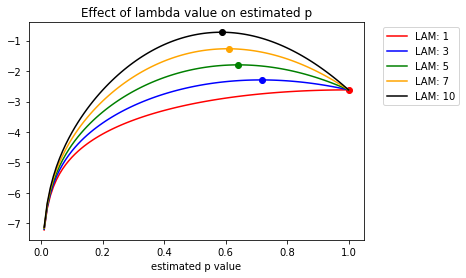
\includegraphics[scale=.75]{./pics/lam-effect.png}
        \caption[Effect of $\lambda$]{Effect of different values of $\lambda$ on estimated $p$ value. The large point on each line is the maximum value, and reflects the returned estimated $p$ of a headline}
        \label{fig:lam-effect}
    \end{center}
\end{figure}

The previous steps give estimators $S$ and $O$. Using these, we are able to estimate the sentiment score $p$ for a new headline that is not in the training sample. Using model \ref{multinom}, we estimate $p$ using Maximum Likelihood Estimation. This is simply testing values in some range and determining which value gives the maximum output. We also include penalty term $\lambda \log(p(1-p))$ and finish with the following optimisation:

\begin{equation}
\widehat p = \arg \max_{p \in [0,1]} \left\{ \widehat s^{-1} \sum_{j \in S} \log (p O_{+,j} + (1-p) O_{-,j}) + \lambda \log(p(1-p)) \right\}
\end{equation}

\noindent
where $\widehat s$ is the total count of word from $S$ in the new headline, $d_j, O_{+,j}, O_{-,j}$ are the entries for word $j$ in the corresponding vectors and $\lambda$ is a tuning parameter that ensures that the majority of headlines are neutral by pushing the estimate towards a neutral sentiment score of 0.5. The effect of lambda is shown in figure \ref{fig:lam-effect}


% \section{Financial Markets and Stock Exchanges}


\section{Portfolios and Financial Market Analysis}
\label{sec:portfolios-analysis}
Evaluating word lists generated by any method of sentiment analysis can be done by creating portfolios based on news with the highest positive or negative sentiment and buying the most positive stocks while selling the negative ones. This gives a good indication of the predictive power of a word list.

\subsection{Portfolios}
\label{sub:portfolios}
A portfolio is simply a list of stocks that can be invested in by an individual or firm. The returns from a portfolio is defined as the profit accrued from all stocks over a set time period, usually daily, monthly or annually. Due to the nature of stocks, simply listing the returns as a concrete value does not convey the information required. For example, if stock `A' were to be invested in at value \$50, and it rose to \$60 the following day, the returns could be said to be \$10. However, if stock `B' were valued at \$1000, and the following day it rose to \$1010, the monetary value would be equivalent at \$10, but the percentage return is vastly different; 20\% returns for stock `A' and 1\% for `B'. For this reason, returns from portfolios are expressed as a percentage.

Daily returns are usually very slight, as the time period is very small, often being smaller than 1\%. In the interest of readability, \textit{basis points} (also known as bps or bips) are used in lieu of a percentage, where 1 bip is equivalent to 0.01\%. This makes it much easier to represent very small returns as are common in daily returns.

\subsubsection{Creating a portfolio}
\label{ssub:portfolio-creation}
A portfolio is constructed using a number of stocks and can be either bought (taking the `long' position) or sold (taking the `short' position). For stocks that are bought, the returns can be calculated from the difference in price at the time that the stock is sold. More concretely, if a stock has value $S_{t}$ at time $t$, and held for $n$ days before being sold, the long returns in percentage form can be calculated using the following formula:

\begin{equation}
\frac{S_{t+n}}{S_{t}} - 1
\end{equation}

\noindent
Similarly, for short returns, as the stock is being sold, profit is acquired if the stock falls in value, therefore the returns can be calculated using the following formula:

\begin{equation}
\frac{S_{t}}{S_{t+n}} - 1
\end{equation}

\noindent
Of course, these simple formulae neglect transaction fees that can apply when constructing real portfolios. However, as we are creating portfolios in a theoretical sense, this suits our needs.

Once the portfolio has been constructed, the weighting for each stock must be considered. Each portfolio will have a value, which is the amount of money invested into it, and each stock will in turn get an investment that is a percentage of this overall value. There are three major strategies that can be used to construct a portfolio: equal weighting, price weighting, and value weighting. Each strategy has its own unique set of advantages and disadvantages.

The equal weighted is perhaps the simplest of these strategies: if a portfolio is comprised of $n$ stocks and has some investment $v$, each stock has $v/n$ invested into it. This strategy glosses over differences in stock size or price.

Price weighted portfolios assign much more money to stocks with higher value associated to them. This can be calculated in a number of ways, but the way we calculate this is if stock $s_i$ in portfolio $P = [s_1, \dots, s_n]$ has market value $P_{i,t}$ at time $t$, the weight of stock $s_i$ would be:

\begin{equation}
w_{i,t} = \frac{P_{i,t}}{\sum_{n}^1 P_{n,t}}
\end{equation}

\noindent
The amount invested into stock $s_i$ at time $t$ would then be $w_{i,t} \times v$.

Finally, value weighted portfolios combine both the price of the stock with the number of outstanding stocks, which creates a much larger bias towards large companies. As before, if stock $s_i$ in portfolio $P=[s_1, \dots, s_n]$ has market value $P_{i,t}$ at time $t$, and has $s_o$ outstanding stocks, the weight of stock $s_i$ is:

\begin{equation}
w_{i,t} = \frac{P_{i,t} \times s_o}{\sum_{n}^1 P_{n,t}}
\end{equation}

Equal weighted stocks more closely resemble hedge funds, as well as being the case that smaller companies are able to more quickly encapsulate market share and investor interest. Equal weighted investments ensure a portfolio has a higher representation of smaller stocks, at the higher risk of the stock failing. Conversely, value weighted portfolios tend to be safer, as they prioritise larger companies that are more stable. The downside to utilising this method is that the large percentage increases observed in smaller stocks will have less effect, and therefore some profit can be lost. Price weighted construction lies somewhere in the middle of the two, being relatively simple to construct, as with equal weighting, but with slight consideration to the price of a stock. The downside of this construction is that the weights assigned are somewhat arbitrary as the price of a stock can fluctuate greatly.

\subsection{Evaluating a portfolio}
To successfully determine the success of a portfolio, it is not always as simple as observing the profit alone. While this is a good indicator of the potential returns that could be gleaned from a given portfolio or investment method, it is important to consider external factors and risks that may be involved. The following methods are used to provide more insight into an investment method.

\subsubsection{Sharpe Ratio}
\label{ssub:sharpe-ratio}
William Sharpe created the Sharpe ratio in 1966 and is one of the most referenced comparison of risk versus return in finance \parencite{sharpe-ratio}. The formula for this ratio is exceedingly simple --- one of the key factors in its wide usage --- and is as follows:

\begin{equation*}
S(x) = \frac{r_x - R_f}{\sigma(r_x)}
\end{equation*}

\noindent
where $x$ is the investment, $r_x$ is the average rate of return of $x$, $R_f$ is the risk free rate of return, and $\sigma(r_x)$ is the standard deviation of $r_x$. The risk free rate of return is simply the theoretical rate of return on an investment with absolutely no risk. Subtracting these risk free returns from the average rate of returns of $x$ yields the true rate of returns.

The value of an investment's Sharpe ratio measures the performance with adjustment for risk: the higher the ratio, the better the performance of the investment when adjusted for risk. As a reference, a ratio of 1 or higher is good, 2 or better is very good, and 3 or better is excellent. 

\subsubsection{Fama French 3 and 5 Factor Models}
\label{ssub:fama-french}
Eugene Fama and Kenneth French co-authored a 1992 paper detailing risk factors in returns on both stocks and bonds. This extends the work Sharpe completed on the Sharpe ratio and goes further in exploring risk factors in returns, along with the capital asset pricing model (CAPM) \parencite{ff3}. CAPM is used for describing systematic risk and expected return, especially for that in stocks. The equation for this is:

\begin{equation}
ER_i = R_f + \beta_t (ER_m - R_f)
\end{equation}

\noindent
where $ER_i$ is the expected return of the investment, $R_f$ is the risk free rate, $\beta_i$ is the beta of the investment and $ER_m - R_f$ is the market risk premium. The beta of an investment is the volatility compared to the rest of the market. It encompasses the sensitivity of a stock to changes in the market. In essence, this gives the expected returns of an asset based on systematic risk. Building on this, Fama and French observed two additional risk factors: the size premium of an asset, or small minus big (SMB), and the value premium, or high minus low (HML). SMB is used to account for companies with small value stocks that generate high returns, while HML accommodates for stocks with equity that is valued cheaply compared to its book value that generate higher returns in comparison to the rest of the market. These factors are used in conjunction to provide the following formula for the Fama French 3 factor model (FF3 model):

\begin{equation*}
ER_i = R_f + \beta_1(ER_m -R_f) + \beta_2 (SMB) + \beta_3(HML) + \alpha
\end{equation*}

The values for SMB and HML are available from French's website \parencite{french_2022}, and can be collected for daily, monthly, or yearly returns. Computing this model on a series of returns from a portfolio gives useful information on the nature of the returns, since the model explains part of the returns. The values for the $\beta$s detail the exposure to each of the risk factors while the $\alpha$, or the intercept, refers to the amount that a portfolio outperformed the expectations of the FF3 model. This alpha is representative of the amount of private or new information that is external from the market and is utilised to construct the portfolio. This means that more simplistic methods of selecting portfolios will not have any private information and therefore the intercept will be much close to zero while a more complicated model will have a larger intercept as simple methods have profits that can be explained by these risk factors.

This model was then revisited by Fama and French in 2015 where they observed two additional factors: robust minus weak (RMW) and conservative minus aggressive (CMA) \parencite{ff5}. RMW corresponds to the profitability of an asset, in that it is the difference between returns of robust or high and weak or low operating profitability. CMA corresponds to the investment factor, and is the difference between returns of conservatively investing firms versus aggressively investing firms, giving the updated formula:

\begin{equation}
ER_i = R_f + \beta_1(ER_m -R_f) + \beta_2 (SMB) + \beta_3(HML) + \beta_4(RMW) + \beta_5(CMA) + \alpha
\end{equation}

%TODO: potentially stick in stuff about momentum factor


% \section{What to do}
% \noindent
% This chapter is intended to describe the background on which execution of the project depends. This may be a technical or a contextual background, or both. The goal is to provide a detailed explanation of the specific problem at hand, and existing work that is relevant (e.g., an existing algorithm that you use, alternative solutions proposed, supporting technologies).  

% Per the same advice in the handbook, note there is a subtly difference from this and a full-blown literature review (or survey).  The latter might try to capture and organise (e.g., categorise somehow) \emph{all} related work, potentially offering meta-analysis, whereas here the goal is simple to ensure the dissertation is self-contained.  Put another way, after reading this chapter a non-expert reader should have obtained enough background to understand what \emph{you} have done (by reading subsequent sections), then accurately assess your work against existing relevant related work.  You might view an additional goal as giving the reader confidence that you are able to absorb, understand and clearly communicate highly technical material and to situate your work within existing literature.







% -----------------------------------------------------------------------------

\chapter{Project Execution}
\label{chap:execution}

% \subsection{Generating the sample}
% \begin{itemize}
%       \item Discuss aligning hte article with returns
%       \begin{itemize}
%             \item Discuss private stocks and public stocks
%             \item Discuss non market days
%       \end{itemize}
%       \item Discuss pre processing the data
%       \item Discuss the kaggle sample
% \end{itemize}
In this section, we present the execution of the project, giving an overview of the dataset used, the configurations of hyperparameters and programming completed. The main idea of the project is to gather a dataset of headlines over a given time period and implement and analyse the algorithm presented by Ke et al. in their 2019 paper \cite{sestm}. Due to the difference in language used in headlines compared to that used in headlines, slightly different approaches were considered for some of the steps, but the theory behind the model remains unchanged.

\section{Project Components}
For this project, I opted to use Jupyter notebook as a base on which to implement the data processing, model training and validation, and portfolio formation. The modular nature of Jupyter, combined with Python's wide range of useful libraries facilitated the creation of this model. Creating each section as an independent cell allows for rigorous debugging and testing of each individual part, which would otherwise be extremely time consuming to test. The full notebook along with accompanying datasets can be found on GitHub \cite{github}.

\section{Dataset and Pre-Processing}
The dataset used for training and validation is available from Kaggle\footnote{\url{https://www.kaggle.com/datasets/miguelaenlle/massive-stock-news-analysis-db-for-nlpbacktests}} and is a collection of around 1.4 million headlines for 6000 stocks from 2009 to 2020. Each headline has the date published, and the ticker that the headline concerns. Some headlines have multiple tickers associated with them, but each ticker-headline combination is a unique entry in the dataset.

The first challenge is to align these headlines with the relevant three day returns, and this was achieved using the Yahoo Finance python library.\footnote{\url{https://pypi.org/project/yfinance/}} Once again, this relates to market close on day $t-2$ to close on day $t+1$ for a headline released on day $t$ (between 4pm on day $t-1$ to 4pm on day $t$). Some headlines are released on non-market days (such as weekends), and for these edge cases, the next available market day is selected as day $t$, and then the previous market day from this new day $t$ is defined as day $t-1$. Similarly, for market days where $t+1$ would fall on a non-market day, the next available market day is defined as day $t+1$. As many headline are released each day, computing the returns for each unique headline in this way would create significant redundancy, and therefore for each unique stock in the dataset, market data for the entire 11 year timespan is pulled in order to create a lookup table. Then, as opposed to calculating the stock values for each headline, if a headline is released on day $t$ relating to stock $s$, the open and close values can be retrieved via the key $(s,t)$. Finally, each headline is iterated through, assigning the appropriate market close values from the lookup table, and stored in json format for future usage. An example json entry is shown below in listing \ref{json} where `open' refers to market value of a ticker day $t-1$ and `close' refers to market value on day $t+1$.

\begin{lstlisting}[float={t},caption={Example JSON headline entry},label={json},language=c]
      {
            "headline": Barclays Maintains Equal-Weight on Agilent
            Technologies, Lowers Price Target to $76
            "date": 2020-03-26
            "ticker": A
            "mrkt_info": {
                  "open": 67.0
                  "close": 70.9100036621
            }
      }
\end{lstlisting}

\begin{lstlisting}[float={t},caption={Creating lookup table},label={lookup-table},language=Python]
day_t_data = {}
TOTAL_ARTS = len(stock_data)
for t in stock_data:
      # iterate through each ticker, and gather day t-1 (from_stock), 
      # day t and day t+1 (to_stock) data for ease of lookup
      #
      # to get day t: day_t_data[t][date]['day_t']
      ticker_date_data = {}
      start = min(stock_data[t].index)
      end = max(stock_data[t].index)
      curr_date = start
      while curr_date < end:
            day_t = curr_date
            while (not (day_t in stock_data[t].index) and day_t <= end):
                  day_t += dt.timedelta(days=1)
            from_stock = day_t - dt.timedelta(days=2)
            to_stock = day_t + dt.timedelta(days=1)
            while (not (from_stock in stock_data[t].index) and from_stock >= start):
                  from_stock -= dt.timedelta(days=1)
            while (not (to_stock in stock_data[t].index) and (to_stock <= end):
                  to_stock += dt.timedelta(days=1)
            if(from_stock > start and to_stock < end):
                  ticker_date_data[curr_date] = {
                        'day_t': day_t,
                        'from_stock': stock_data[t]['Close'][from_stock], 
                        'to_stock': stock_data[t]['Close'][to_stock]
                  }
            curr_date += dt.timedelta(days=1)
      day_t_data[t] = ticker_date_data
\end{lstlisting}

Note that some tickers do not have publicly available stock market information for the entire span of the sample. This is due to some companies being private for the duration, or turning private, meaning that their information is not accessible through standard means. Headlines aligned with these private tickers are removed from the sample, leaving around 1 million articles in the sample.

With the headlines aligned to the appropriate returns, the text data must be preprocessed to allow for successful and efficient semantic analysis. Taking the text content of each headline, the following transformations are applied, also detailed by figure \ref{fig:pre-processing-flow}:

\begin{figure}[!ht]
      \centering
      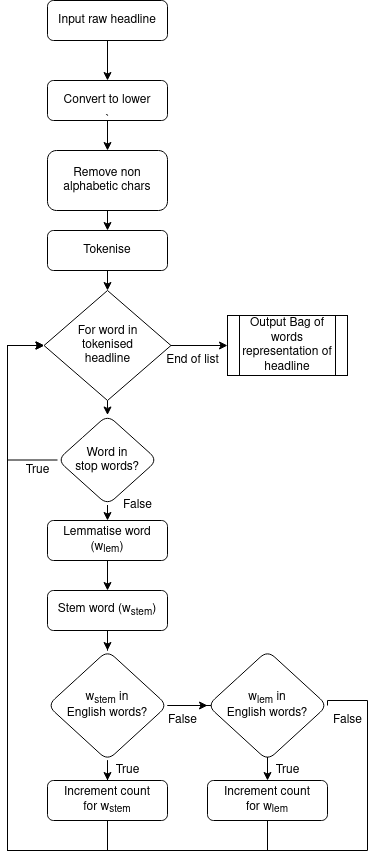
\includegraphics[scale=.6]{./pics/pre-processing-flowchart.png}
      \caption[Bag of words flowchart]{Flowchart showing conversion of raw headline into bag of words format}
      \label{fig:pre-processing-flow}
\end{figure}

\begin{itemize}
      \item Convert the headline to lower case. This is to ensure that different cases do not lead to multiple entries of the same word, differing only by letter captialisation.
      \item Remove non alphabetic characters
      \begin{itemize}
            \item Spaces are retained to allow for tokenisation
      \end{itemize}
      \item Tokenise the headline (convert to list of words)
      \item Remove non-English words \footnote{The list of English words is available from item 106 from \url{https://www.nltk.org/nltk_data/}}
      \item Remove stop words. \footnote{The list of stopwords used is from item 86 from \url{https://www.nltk.org/nltk_data/}} Stop words are a term used in NLP to describe very commonly used words that are unimportant (such as `and' or `the'). They serve only as noise and are removed to allow focus on more important news.
      \item Lemmatise each word (for example converting `mice' to `mouse' or `skis' to `ski') \footnote{The lemmatisation process uses WordNet (item 106) from \url{https://www.nltk.org/nltk_data/}}
      \item Stem each word (for example, `regional' to `region').\footnote{The stemming process uses Snowball stemmer from wordnet from \url{https://www.nltk.org/nltk_data/}} Note that as stemming aims to create the most general stem of a word, it sometimes leaves a word that is not English (such as `easily' to `easili'). For this reason, if the stemmed word is not in the list of English words, but the lemmatized word is, then this word is not stemmed.
      \item Convert to bag of words (BOW) representation (list of unique words with associated word counts for a given headline)
\end{itemize}

By utilising stemming where appropriate (i.e. when the stemmed word is included in the list of English words), we ensure that the resulting bag of words most closely resembles the original headline, while also grouping words that are similar by root. This helps to keep sentment consistent, as the root of a word is likely to be what holds sentiment, rather than the form it is used in. Another complication is the part of speech according to which a word is lemmatised. For example, the word `trying' is both a noun and a verb, depending on context (e.g. `a \textit{trying} quarter' versus `I was \textit{trying} really hard'). The lemmatisation of this word in the context of a noun is `trying', in verb context is `try' and the stem is `tri'. By default, the Wordnet Lemmatizer assumes the input is a noun, and I decided to do the same, at the potential risk of misclassifying a word. However, the shortcomings of treating each word as a noun are often covered by the stemming of the word, therefore using the two in conjunction gives the most accurate root of a word.


\section{Training the Model}
\label{sec:training-model}
Using the BOW representation of each of the headlines, the data is able to be processed according to the algorithm outlined by Ke et al. In the spirit of the original paper, the dataset is divided up into 17 three year training and validation windows, where two years are used for training a model, and the final year is used for validation purposes. More concretely, the training sample begins in 2010-01-01 and ends on 2017-12-31, the validation sample begins in 2012-01-01 and ends in 2018-12-31, leaving articles between 2019-01-01 and 2020-06-08 as an out of sample dataset used for testing the robustness of the model. All the computation is completed on this window, and then it is moved forward four months and repeated in a rolling window method.

\begin{table}[t]
\centering
\begin{tabular}{c>{\rowmac}c>{\rowmac}c>{\rowmac}c>{\rowmac}c>{\rowmac}c>{\rowmac}c>{\rowmac}c<{\clearrow}}
\toprule
Window start date & $|S|/2$ & $\alpha_+$ & $\alpha_-$ & $\kappa$ & $\lambda$ & Minimum error & Avg Min Error\\
\midrule
2010-1-1 & 100 & 0.0529 & 0.0487 & 92 & 5 & 20402.2 & 0.24727\\
2010-5-1 & 100 & 0.0405 & 0.0384 & 94 & 5 & 20714.66 & 0.24926\\
2010-9-1 & 25 & 0.1116 & 0.1043 & 92 & 5 & 20426.81 & 0.24675\\
2011-1-1 & 25 & 0.1023 & 0.1064 & 92 & 1 & 19963.67 & 0.24574\\
2011-5-1 & 50 & 0.1002 & 0.0921 & 90 & 5 & 19075.08 & 0.24598\\
2011-9-1 & 100 & 0.0425 & 0.0404 & 94 & 5 & 19255.78 & 0.24653\\
2012-1-1 & 100 & 0.0754 & 0.0744 & 88 & 5 & 20474.7 & 0.24744\\
2012-5-1 & 100 & 0.051 & 0.0489 & 92 & 10 & 21839.81 & 0.24961\\
2012-9-1 & 100 & 0.0536 & 0.0473 & 92 & 10 & 22243.55 & 0.24931\\
2013-1-1 & 50 & 0.0536 & 0.0672 & 94 & 5 & 21546.5 & 0.24702\\
\setrow{\bfseries}*2013-5-1 & 100 & 0.084 & 0.0913 & 86 & 5 & 22095.56 & 0.24552\\
2013-9-1 & 100 & 0.0688 & 0.076 & 88 & 10 & 23415.73 & 0.24885\\
2014-1-1 & 100 & 0.0395 & 0.0375 & 94 & 5 & 24819.11 & 0.24818\\
2014-5-1 & 100 & 0.0823 & 0.0954 & 86 & 5 & 24060.98 & 0.24652\\
2014-9-1 & 100 & 0.0392 & 0.0412 & 94 & 5 & 23536.73 & 0.24904\\
2015-1-1 & 100 & 0.0778 & 0.0898 & 86 & 5 & 22801.46 & 0.24805\\
2015-5-1 & 100 & 0.0471 & 0.0571 & 92 & 5 & 23642.32 & 0.24871\\
2015-9-1 & 100 & 0.0603 & 0.0734 & 90 & 5 & 26361.23 & 0.24772\\
2016-1-1 & 100 & 0.0478 & 0.0518 & 92 & 5 & 29950.54 & 0.24818\\
\bottomrule
\end{tabular}
\caption[Model configurations]{Best configuration and error for each window. Smallest error window highlighted in \textbf{bold}}
\label{min-error-train}
\end{table}

\begin{lstlisting}[float={!htb},caption={Calculating list of sentiment words},label={lst:calc-sentiment},language=Python]
kappa_configs   = [86, 88, 90, 92, 94]
alpha_configs   = [25,50,100]
# fraction of positively tagged training articles
train_pi = sum(sgn_i > 0 for sgn_i in train_sgn)/len(train_sgn)
for alpha in alpha_configs:
      for KAPPA in kappa_configs:
      #TRAINING
      kappa_percentile = np.percentile(np.array(list(total_j.values())),KAPPA)
      # return the nth percentile of all appearances for KAPPA

      #calculate alpha vals
      ALPHA_PLUS  = train_pi/2
      ALPHA_MINUS = train_pi/2
      delta_plus  = train_pi/4
      delta_minus  = train_pi/4
      # set limit on max iterations
      delta_limit = 0.0001
      
      while(delta_plus > delta_limit):
            no_pos_words = len([w for w in total_j if f[w] >= train_pi + ALPHA_PLUS and total_j[w] >= kappa_percentile])
            if no_pos_words == alpha:
                  # alpha plus found
                  delta_plus = 0
            elif (no_pos_words > alpha):
                  ALPHA_PLUS += delta_plus
                  delta_plus /= 2
            else:
                  ALPHA_PLUS -= delta_plus
                  delta_plus /= 2
      while(delta_minus > delta_limit):
            no_neg_words = len([w for w in total_j if f[w] <= train_pi - ALPHA_MINUS and total_j[w] >= kappa_percentile])
            if no_neg_words == alpha:
                  # alpha minus found
                  delta_minus = 0
            elif (no_neg_words > alpha):
                  ALPHA_MINUS += delta_minus
                  delta_minus /= 2
            else:
                  ALPHA_MINUS -= delta_minus
                  delta_minus /= 2
      sentiment_words = [w for w in total_j if ((f[w] >= train_pi + ALPHA_PLUS or f[w] <= train_pi - ALPHA_MINUS) and total_j[w] >= kappa_percentile)]
\end{lstlisting}

The training section employs the screening (section \ref{screen-sentiment}) and learning (section \ref{learn-sentiment}) steps, while the validation is the application of the scoring new headlines (section \ref{new-headlines}) step. The validation section is used to consider the hyperparameters ($\alpha_+, \alpha_-, \kappa, \lambda$), and these are evaluated according to a fixed number of possibilities. $\alpha_\pm$ is calculated such that $S$ has either 25, 50, or 100 words of each sentiment (i.e. for the selection of $\alpha = 25$, $|S| = 50$). This is calculated via binary search, assuming $\alpha_\pm = 0.25$ at first. If the resulting set of words is larger than the selected configuration, then $\alpha$ must be larger than the current value, as the larger $\alpha$ is, the fewer words satisfy the condition. Similarly, the inverse for the case where the set of words contains fewer words than desired. $\kappa$ is selected to be the 86, 88, 90, 92 or 94th percentiles of word counts. Note that the $\kappa$ restraint is applied first such that a word is not selected via the $\alpha$ constraint that must then be removed due to the $\kappa$ constraint, leaving $S$ with fewer words than desired. Combining both the calculated $\alpha_\pm$ values and the calculated $\kappa$ value, the list of sentiment words for the training window is compiled, illustrated in listing \ref{lst:calc-sentiment}. Finally, $\lambda$ is selected to be either 1, 5, or 10, for a total of 45 configurations.

Each of these 45 configurations is iterated through for each window, and the $\ell^1$ error is calculated for each, before selecting the setup with minimum error (as this is our loss function). $\ell^1$ error in this case is simply:


\begin{equation}
\sum_{i=1}^{n}|\widehat{p_i} - p_i|
\end{equation}

\noindent
where $\widehat{p_i}$ is the estimated sentiment and $p_i$ is the standardised return rank of article $i$ in the validation set. The loss function of $\ell^1$-norm error was selected for its robustness. The entire process of training and validation takes a considerable length of time and therefore some time was spent optimising the code. A complete list of optimisations can be found in appendix (REFERENCE) %TODO: add optimisation list and reference it


Table \ref{min-error-train} details the results of the completed rolling window training. Due to the nature of news, some validation sets are larger than others, leading to skewed summed $\ell^1$-norm error. To accommodate for this variation is sample size, the error is taken as an average over all headlines in the sample. Window 2011-1-1 has the smallest minimum error, but also has the smallest validation sample size and after controlling for this factor, window 2013-5-1 is has slightly lower error, meaning this is the optimum window.

\subsection{Bigram training}
Naturally, the order in which words appear in a headline can have a profound impact on the sentiment of a word. This can be captured by training the model on \textit{bigrams}, which are sequences of two words, rather than single words alone. This can then be combined with the lexicon of unigrams to provide a clearer insight into the true sentiment of a headline based on the words used.


\begin{lstlisting}[float={!htb},caption={Calculating list of sentiment words},label={lst:bigram-formation},language=Python]
KAPPA_BIGRAM = 90
kappa_percentile_bigram = np.percentile(np.array(list(total_j.values())),KAPPA_BIGRAM)
# return the nth percentile of all appearances for KAPPA_BIGRAM
bigrams_to_remove = []
mutual_info = {}
for w in total_j_bigram:
      component_words = w.split()
      if not (total_j[component_words[0]] >= kappa_percentile_bigram and total_j[component_words[1]] >= kappa_percentile_bigram):
      bigrams_to_remove.append(w)
      else:
      mutual_info[w] = total_j_bigram[w] / (total_j[component_words[0]] * total_j[component_words[1]])
mutual_info_percentile = np.percentile(np.array(list(mutual_info.values())),95)
bigrams_to_remove.extend([w for w in mutual_info if mutual_info[w] <= mutual_info_percentile])
for b in bigrams_to_remove:
      pos_j_bigram.pop(b)
      total_j_bigram.pop(b)
      f_bigram.pop(b)
\end{lstlisting}

The algorithm naturally lends itself to training with bigrams and little is needed in the way of adjustment, as the bigrams are treated the same way as words. The only slight difference is the way that bigrams are filtered out. Due to the nature of bigrams, they will be, on average, far less frequent than unigrams, simply because of the increased number of possibilities. For this reason, centain measures are taken to ensure that only meaningful bigrams are considered. For each window, all articles are divided into bigrams in the same way that the BOW representations are created. Stopwords are not considered for potential bigrams, and as such if two words are separated by a stop word, the resulting bigram would be as if the stop word were absent (e.g. `chalk and cheese' would create the bigram `chalk cheese'). Then, bigrams are removed if either component word is not common (below 85th quantile of word counts). Among the remaining phrases, only those bigrams with mutual information ranking in the top 5\% are retained. Mutual information score is calculated as the ratio of the frequency of the bigram divided by the product of the frequency of the component words. The percentile chosen here is slightly higher than the 1\% used by the original paper, as the dataset contained articles, meaning there are far more bigrams than in the dataset used here. For this reason, I chose to consider a higher number of bigrams to ensure completeness. After this filtering step, the rest of the training continues as before. The preparation for bigrams is shown in listing \ref{lst:bigram-formation}.

\section{Out of Sample Testing}
Using the optimally trained model (shown in table \ref{min-error-train}), the articles not used in either training or validation samples are then used to determine the strength of the model. Each market day $t$, the headlines released from 9 a.m. on day $t-1$ to 9 a.m. on day $t$ are selected and ranked $p$ value calculated from the scoring step (\ref{new-headlines}). Each ticker in the sample is then ranked according to sentiment of related headlines for that day. If a ticker has multiple headlines, the average sentiment from all related headlines is taken for the firm. From this, a portfolio is created, where the top 50 sentiment stocks are bought, and the lowest 50 sentiment stocks are shorted.

Some constraints are placed on the stocks that can be chosen, to ensure that stocks are not bought when they have negative sentiment. For a stock to be bought, it must have $\widehat p_i < 0.5$, and the inverse for a stock to be sold. On the occasion where there are not 50 stocks with positive sentiment, this is to avoid the portfolio purchasing slightly negative stocks, and therefore less than 50 stocks are used in this instance.
%TODO: say why 9 to 9 and not 9.30 (which is market open)


% \section{What to do}


% \noindent
% This chapter is intended to describe what you did: the goal is to explain
% the main activity or activities, of any type, which constituted your work 
% during the project.  The content is highly topic-specific, but for many 
% projects it will make sense to split the chapter into two sections: one 
% will discuss the design of something (e.g., some hardware or software, or 
% an algorithm, or experiment), including any rationale or decisions made, 
% and the other will discuss how this design was realised via some form of 
% implementation.  

% This is, of course, far from ideal for {\em many} project topics.  Some
% situations which clearly require a different approach include:

% \begin{itemize}
% \item In a project where asymptotic analysis of some algorithm is the goal,
%       there is no real ``design and implementation'' in a traditional sense
%       even though the activity of analysis is clearly within the remit of
%       this chapter.
% \item In a project where analysis of some results is as major, or a more
%       major goal than the implementation that produced them, it might be
%       sensible to merge this chapter with the next one: the main activity 
%       is such that discussion of the results cannot be viewed separately.
% \end{itemize}

% \noindent
% Note that it is common to include evidence of ``best practice'' project 
% management (e.g., use of version control, choice of programming language 
% and so on).  Rather than simply a rote list, make sure any such content 
% is useful and/or informative in some way: for example, if there was a 
% decision to be made then explain the trade-offs and implications 
% involved.

% \section{Example Section}

% This is an example section; 
% the following content is auto-generated dummy text.

% \subsection{Example Sub-section}

% \begin{figure}[t]
% \centering
% foo
% \caption{This is an example figure.}
% \label{fig}
% \end{figure}

% \begin{table}[t]
% \centering
% \begin{tabular}{|cc|c|}
% \hline
% foo      & bar      & baz      \\
% \hline
% $0     $ & $0     $ & $0     $ \\
% $1     $ & $1     $ & $1     $ \\
% $\vdots$ & $\vdots$ & $\vdots$ \\
% $9     $ & $9     $ & $9     $ \\
% \hline
% \end{tabular}
% \caption{This is an example table.}
% \label{tab}
% \end{table}

% \begin{algorithm}[t]
% \For{$i=0$ {\bf upto} $n$}{
%   $t_i \leftarrow 0$\;
% }
% \caption{This is an example algorithm.}
% \label{alg}
% \end{algorithm}

% \begin{lstlisting}[float={t},caption={This is an example listing.},label={lst},language=C]
% for( i = 0; i < n; i++ ) {
%   t[ i ] = 0;
% }
% \end{lstlisting}

% This is an example sub-section;
% the following content is auto-generated dummy text.
% Notice the examples in Figure~\ref{fig}, Table~\ref{tab}, Algorithm~\ref{alg}
% and Listing~\ref{lst}.

% \subsubsection{Example Sub-sub-section}

% This is an example sub-sub-section;
% the following content is auto-generated dummy text.

% \paragraph{Example paragraph.}

% This is an example paragraph; note the trailing full-stop in the title,
% which is intended to ensure it does not run into the text.

% -----------------------------------------------------------------------------

\chapter{Critical Evaluation}
\label{chap:evaluation}

\section{Analysis of Word Lists}
\label{sec:word-list-analysis}
\begin{figure}[ht]
\begin{subfigure}[b]{\textwidth}
\centering
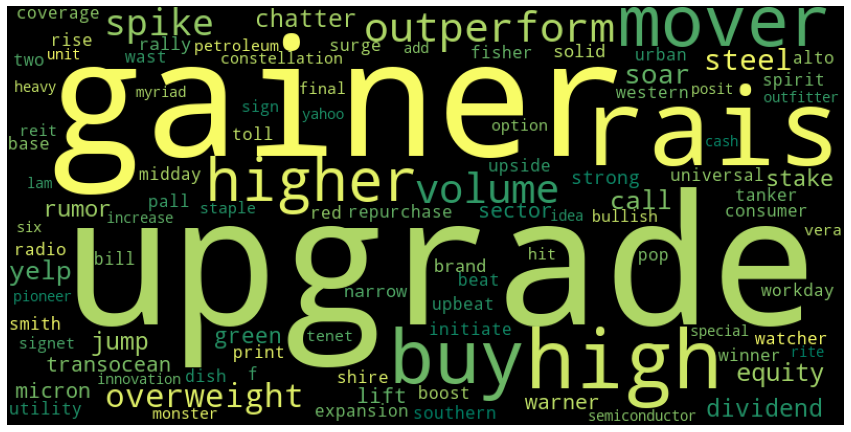
\includegraphics[scale=0.4]{pics/positive.png}
\caption{Positive words}
\end{subfigure}

\begin{subfigure}[b]{\textwidth}
\centering
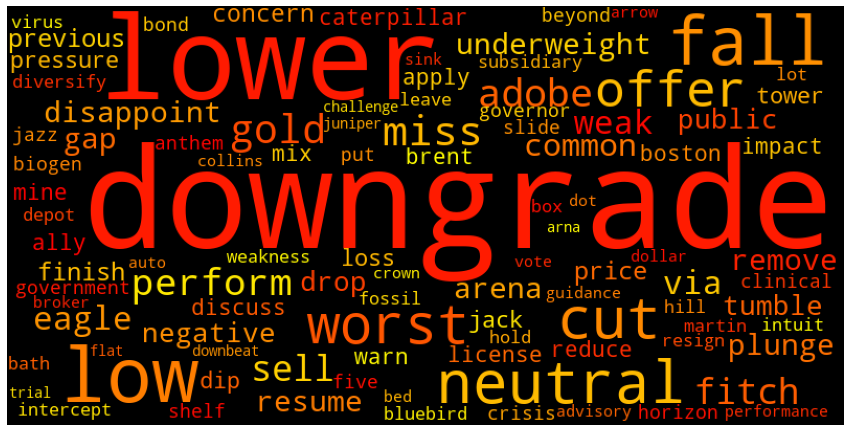
\includegraphics[scale=0.4]{pics/negative.png}
\caption{Negative words}
\end{subfigure}
\caption[Word clouds]{Word clouds demonstrating sentiment charged words. Font size corresponds to average tone across all training samples}
\label{wordclouds}
\end{figure}

Following the construction of matrix $O$, figure \ref{wordclouds} demonstrates the list of sentiment charged words on average over all training 19 windows. At each training and validation window, the sentiment lists are generated completely from scratch, and while there is some overlap, each list can vary significantly. The font size corresponds to the average tone (calculated by $\frac{1}{2}(O_+ - O_-)$) of the words across all windows. Of the top 50 positive sentiment words, the following appeared in at least 15 of the 19 windows, with words highlighted in \textbf{bold} appearing in all windows:
\begin{center}
      \textit{author, rumor, volume, repurchase, rais(e),} \textbf{gainer, mover, high, upgrade}
\end{center}

\noindent
The following words appear in at least 15 of the 19 windows with respect to top 50 negative sentiment words with those highlighted in \textbf{bold} appearing in all windows:
\begin{center}
      \textit{offer, negative, neutral, public, low,} \textbf{miss, lower, loser, cut, fall, weak, downgrade, underweight}
\end{center}

Simply by inspection, each group appears reasonable, in the sense that many of the words with high values in either sentiment could be assumed. However, some words are somewhat surprising and this may offer an insight into subconscious bias that exists in writing headlines as opposed to article bodies. For example, the word \textit{volume} is, under normal circumstances, a sentiment neutral word, but according to the model generated by SESTM, is a highly positive word. Examples of headlines including this word include:
\begin{itemize}
      \item \textit{Agilent spikes to high of \$60.40 on Volume}
      \item \textit{Markets gather some momentum as volume remains light, geopolitical tension improving}
      \item \textit{Tuesday's Mid-day options for volume leaders}
\end{itemize}

Observing these headlines, it is clear that the words are being used in a positive context, and this could be due to subconscious usage of the word when constructing such headlines. However, in any learning based algorithm, overfitting must be considered. Overfitting in this instance refers to a model that is too closely trained to the training sample, meaning incorrect alignment with out of sample data. Included in the sample are headlines from `Benzinga', which is a company that offers realtime news articles \parencite{benzinga-website}, and has a significant quantity of headlines of the form \textit{Benzinga's top upgrades} (around 16,000 headlines from the entire dataset) and \textit{Benzinga's volume} (with around 2,000). To account for this, the addition of bigrams (discussed further in \ref{sub:bigram-analysis}) gives an insight into frequently occurring pairs of words, and helps to isolate context specific sentiment. If a word has a high estimated impact in a bigram, then the majority of the sentiment comes from its co-appearance with its partner word, helping to eliminate such issues.

Some words, such as `rais' are cut off to their stem by the stemming and lemmatisation step (i.e. `rais' from `raise'), as the stem is also an English word. However, such words are likely to be very infrequently used words themselves, and are very unlikely to be used in a headline. These edge cases do not affect the overall predictive quality of the model, as evidenced by the words shown in figure \ref{wordclouds}. The sentiment for each word is still captured in the stem, and each article is processed in the same way, thus there is no sentiment or predictive power lost in this way. There is a slight complication when it comes to comparing the words included in the model to those in the H4 and LM lexicons, as these lexicons do not contain the stemmed words. For this reason, when checking if a word in the trained model exists in either dictionary, each word in either dictionary is preprocessed in the same way discussed in section \ref{sec:pre-processing}

When compared to the Harvard IV and Loughran McDonald dictionaries, we find that the majority of words labelled with sentiment according to our model are not in either dictionary. The negative sentiment words have much higher overlap, with 13 of the top 50 words appearing in the LM dictionary, while only 3 appear in the H4. Conversely, only 6 words overlap LM in the positive tone, while 5 words overlap the H4 dictionary. Furthermore, many words that are included in either dictionary are determined to be sentiment neutral by the model. This is because the model is trained on a sample of headlines and the vocabulary used in headlines is vastly different to that in everyday use or 10-k filings in the case of LM. Headline vocabulary often contains much more impactful words, as it is intended to be a punchy, attention grabbing piece of text. Often, words that are typically used in headlines are rarely found outside of the context of headlines \parencite{language-newspapers}. For this reason, the lexicons of the model, and that of H4 and LM differ significantly.

\subsection{Bigrams}
\label{sub:bigram-analysis}
The order in which words appear in can have a profound effect on the sentiment of a word. This order sentiment can be captured by exploring the dictionary when constructed from \textit{bigrams} as opposed to unigrams alone. By combining both of these dictionaries, it is possible to gain a clearer understanding of the true sentiment of a headline. Many of the frequently  words unigrams also appear in the bigram. This is partly due to the mutual information restriction on the bigrams consiered by the model, but also because still carry sentiment in combination with other words. Furthermore, somewhat surprisingly there are bigrams that appear in every training window. The headlines in this dataset have an average wordcount of 6.11 (excluding stopwords and non-English words), and therefore one may expect that there would be very few repeating bigrams, which is not the case. This signifies that headline writers may subconsciously use certain combinations of words to convey either positive or negative sentiment

The following bigrams appear positively in at least 13 of the 19 training windows, with those highlighted in \textbf{bold} appearing in all headlines:
\begin{center}
\textit{micron technology, repurchase program, spike higher,} \textbf{volume mover}, \textbf{week high}
\end{center}

The following bigrams appear negatively in at least 14 of the 19 training windows, with those highlighted in \textbf{bold} appearing in all headlines:
\begin{center}
      \textit{general dynamic, bath beyond, bed bath, sector perform, secondary offer, week low, resume trade, offer common,} \textbf{public offer}
\end{center}

Several of the high frequency unigrams do not appear in the high frequency bigrams, indicating that the sentiment carried by these words is not tied to context, for example raise for positive and weak for negative. Due to the nature of the headlines, the model also picks up on especially highly or poorly performing companies, and this is sometimes reflected in the generated word lists. For example, `\textit{bed bath}' and `\textit{bath beyond}' both appearing in the negative bigram list is almost certainly a result of the poor performance of the company \textit{Bed, Bath and Beyond}, whose stock prices stagnated and then fell from mid 2013 \parencite{bed-bath-yahoo}. Also seen in figure \ref{wordclouds}, Adobe is likely to be in reference to the company `Adobe'.


\section{Daily returns}
\label{sec:daily-returns-analysis}

\begin{table}[!ht]
\begin{center}
\begin{tabular}{lccccccc}
      \toprule
      & Sharpe &  Average & Daily & \multicolumn{2}{c}{FF3} & \multicolumn{2}{c}{FF5} \\
      \cmidrule(lr){5-6}
      \cmidrule(lr){7-8}
      % \cmidrule(lr){9-10}
      Formation & Ratio & Return & Turnover & $\alpha$ & $R^2$ & $\alpha$ & $R^2$ \\
      \midrule
      EW LS & 0.84 & 9.23 & & 5.59 & 4.11\% & 5.57 & 4.16\% \\
      EW L & 0.69 & 9.75 & & 6.56 & 21.62\% & 5.86 & 23.0\% \\
      EW S & -0.09 & -0.53 & & -1.66 & 25.71\% & -0.98 & 26.68\% \\
      VW LS & 0.56 & 6.31 & & 4.73 & 0.83\% & 7.16 & 4.58\% \\
      VW L & 0.86 & 10.47 & & 6.51 & 34.3\% & 7.55 & 35.16\% \\
      VW S & -0.38 & -4.16 & & -2.48 & 32.54\% & -1.08 & 34.08\% \\
      \bottomrule
\end{tabular}
\caption{Performance of Daily News Sentiment Portfolios one day ahead}
\label{portfolio-performance}
\end{center}
\end{table}

Using the headlines that were saved for out of sample testing, a portfolio is constructed for each day. On average, 358 firms have articles linked to them on a given day, and of these, almost three quarters of these firms have headlines containing one or more sentiment words (are not marked neutral by the model). According to the constraints ($\widehat p_i < 0.5$ for a stock to be bought, and vice versa for a stock to be sold), there are some days where less than 100 stocks form the portfolio, in which case we trade with the largest value possible. On average, the long side trades with 49.5 stocks, while the short side has 48, so the model trades at very close to 100 stocks the majority of the time.

Table \ref{portfolio-performance} describes the performance of the constructed portfolios. The long-short portfolio is a zero-net-investment portfolio, which is a theoretical portfolio that requires zero investment, as it buys the same value of stocks as it sells \parencite{zero-net}. The portfolio is theoretical as a true zero-cost investment is impossible in practice for a number of reasons, one of which being that to sell a stock and profit from the decline, there is collateral from the loan from the broker. However, for the purposes of the following experiments, it is sufficient. The two investment methods (equal and value weighted) are split up into the long-short combined portfolio (L-S), and the long (L) and short (S) legs are also displayed separately for comparison purposes. The daily turnover section displays the average turnover each day, which would be 100\% as the profit is liquidated at the end of each day, but some stocks are retained the following day. A turnover of 90\% (as in VW L) implies that on average 1 in 10 stocks are retained the following day. This could be due to headlines or news articles that are concerning the same events (stale news), or repeat sentiment headlines as a story unfolds over a number of days.

The Sharpe ratio refers to the calculated annualised sharpe ratio and this reflects the ratio of profit versus risk. Sharpe ratios are annualised by multiplying the daily sharpe ratio (shown in \ref{ssub:sharpe-ratio}) by $\sqrt{252}$ as this is the number of trading days in a year, and will give a clearer image of the risk involved in the potential profit.

The FF3 and FF5 sections refer to Fama French 3 and 5 factor regression respectively, while the $\alpha$ concerns the intercept. The $\alpha$ value reflects how much the output outperformed the expected value calculated by the factors in the model and is generated by privately created information, or information that is not available in the market. In other words, if the $\alpha$ is a very small percentage of the generated returns, then the returns that an investment has generated can be explained by regular movement in the markets, and there is no private information that is being used to generate profit. The $R^2$ value is the measure of the proportion of variance that is for the dependent variable (in this case, daily returns for the portfolio) is explained by the independent variables (in this case, the Fama French factors discussed in \ref{ssub:fama-french}). Therefore, if $R^2 = 25\%$, then around a quarter of the observed variation can be explained by the inputs. In terms of an investment, this corresponds to the percentage of movement that can be explained by movements in the independent variables.

This figure clarifies two key facts: firstly, most of the formations generate a slight profit with a fair amount of risk, reflected in the Sharpe ratios. None of the formations have a Sharpe ratio of $>1$, meaning each of the portfolios carry significant risk. The second fact is that the equal weighted portfolio outperforms the value weighted portfolio overall, while the value weighted portfolio sees a slight performance on the long side.

\begin{figure}[!t]
      \centering
\begin{tikzpicture}
\begin{axis}[scale only axis, height=8cm, width=\textwidth*.9, grid=both,
      legend pos=north west,
      date coordinates in=x, date ZERO=2019-01-01, xticklabel=\month-\year,ymin=-50,ymax=75,
      xtick={2019-01-01,2019-02-01,2019-03-01,2019-04-01,2019-05-01,2019-06-01,2019-07-01,2019-08-01,2019-09-01,2019-10-01,2019-11-01,2019-12-01,2020-01-01,2020-02-01,2020-03-01,2020-04-01,2020-05-01,2020-06-01},
      xticklabel style={
            rotate=60,
      },
       xmin=2019-01-01,
       xmax=2020-06-08]
\addplot [red, very thick, mark=none] table [header=true,x=date,y=EW-L, col sep=comma]{data/one-day-ahead.csv};
\addplot [blue, very thick, mark=none] table [header=true,x=date,y=EW-S, col sep=comma]{data/one-day-ahead.csv};
\addplot [black, very thick, mark=none] table [header=true,x=date,y=EW-LS, col sep=comma]{data/one-day-ahead.csv};
\addplot [red, very thick, dotted, mark=none] table [header=true,x=date,y=VW-L, col sep=comma]{data/one-day-ahead.csv};
\addplot [blue, very thick, dotted, mark=none] table [header=true,x=date,y=VW-S, col sep=comma]{data/one-day-ahead.csv};
\addplot [black, very thick, dotted, mark=none] table [header=true,x=date,y=VW-LS, col sep=comma]{data/one-day-ahead.csv};
% \draw ({axis cs:2020-03-11,0}|-{rel axis cs:0,0}) -- ({axis cs:2020-03-11,0}|-{rel axis cs:0,1})
 \draw[green, very thick] (axis cs: 2020-03-11,\pgfkeysvalueof{/pgfplots/ymin}) -- 
                      (axis cs: 2020-03-11,\pgfkeysvalueof{/pgfplots/ymax})node[anchor=west,rotate=90]{Coronavirus declard pandemic};
                
\legend{L EW, S EW, LS EW, L VW, S VW, LS VW}

\end{axis}
\end{tikzpicture}
\caption[Daily cumulative log returns]{Cumulative log returns for each formation over the out of sample headlines}
\label{graph-returns}
\end{figure}


Figure \ref{graph-returns} details the cumulative log returns over the entire out of sample dataset. Here, The performance of each of the legs are relatively steady in their respective directions until March 2020. At this point, the profits of the short legs skyrocket, while that of the long section plummet --- especially for the value weighted portfolios. This is due to the Coronavirus outbreak, as it was officially declared a pandemic on March 11 2020, indicted by the vertical green line on the graph. Due to lockdown restrictions imposed wordwode, the stock market experienced one of the worst crashes, and was felt particularly by large stocks, before recovering a short while later. The markets began feeling the effect of the lockdown in February 2020, and the crash peaked in March 2020, before beginning to recover in late April \parencite{covid-impact}. This crash can be clearly seen in the affected profits, as the long side suffers significantly, while the short side succeeds greatly. This is simply due to the vasy majority of stocks falling in value, therefore shorting almost any stocks during this time would result in a profit. The extreme disparity in profit for the long side also clearly highlights a limitation with all lexicon based sentiment analysis methods, whether they use supervised learning signals, or use a manually labelled dictionary: they are unable to adapt to rapid changes. Since the COVID-19 virus did not exist during the training and validation samples, the model has no information on the sentiment of headlines that would discuss this, and would ignore it. Naturally, if the model was retrained using data from this time period, it would be able to detect such headlines in the future, but the crux of the issue is that it is impossible to obtain enough information to allow the model to react to such drastic changes in the market.

Graph \ref{graph-returns} reveals slightly different information than that in table \ref{portfolio-performance}. Here, the long side of the value weighted graph is shown to outperform the equal weighted counterpart considerably, before taking a substantial fall during the pandemic induced market crash. On the other hand, the short sides of both weighting strategies fare similarly, until after the crash, where the equal weighted short side experiences a higher spike in profit. Clearly, SESTM is capable of predicting a positive shift in stocks on a one-day-ahead principle, shown by the positive returns in the graph. It is more successful when predicting larger stocks, as value weighed portfolios are influenced more by larger stocks. This represents SESTM's success in detecting positive sentiment in headlines concerning these large firms, which is likely due to increased coverage. As previously discussed, the primary goal for a headline is to capture as much information about the main article body as possible while the secondary goal is to attract the reader to click on the article. For this reason, the headline is far more likely to contain information about more well known stocks, as this satisfies the secondary goal of garnering clicks: if the headline's content is about a stock that is known to the reader, it is more likely that the rest of the article is read.

The two short formations perform very similarly, with both making slight losses. This contradicts the claims made concerning headlines containing more information about large stocks somewhat, although I believe this is due to a different matter. \textcite{linguistic-effect-success} explore the success of a headline based on linguistic features, and conclude that the presence of positive-emotion words is negatively associated with the success of a headline (in terms of popularity), while the inverse is true for negative-emotion words. For this reason, if there is ambiguity on the potential future of a stock, a headline is more likely to take the negative approach, as it is more likely to be successful. In other words, if a news article is mostly neutral, the headline is more likely to contain negative-emotion words, as this garners more views. As a result, the negatively tagged words are less reliable than their positive tagged counterparts, which be one possbile explanation for the lack of profit made by either short formation.

\begin{table}[!ht]
\begin{center}
\begin{tabular}{lccccccc}
      \toprule
      & Sharpe &  Average & Daily & \multicolumn{2}{c}{FF3} & \multicolumn{2}{c}{FF5} \\
      \cmidrule(lr){5-6}
      \cmidrule(lr){7-8}
      Formation & Ratio & Return & Turnover & $\alpha$ & $R^2$ & $\alpha$ & $R^2$ \\
      \midrule
      EW LS & 0.84  & 9.23 & & 5.59 & 4.11\% & 5.57 & 4.16\% \\
      EW L  & 0.69  & 9.75 & & 6.56 & 21.62\% & 5.86 & 23.0\% \\
      EW S  & -0.09 & -0.53 & & -1.66 & 25.71\% & -0.98 & 26.68\% \\
      VW LS & 0.56  & 6.31 & & 4.73 & 0.83\% & 7.16 & 4.58\% \\
      VW L  & 0.86  & 10.47 & & 6.51 & 34.3\% & 7.55 & 35.16\% \\
      VW S  & -0.38 & -4.16 & & -2.48 & 32.54\% & -1.08 & 34.08\% \\
      \midrule
      \multicolumn{8}{c}{Excluding market crash} \\
      \midrule
      EW LS & 0.66  & 6.51 & & 5.52 & 2.24\% & 4.16 & 4.51\% \\
      EW L  & 0.64  & 5.46 & & 1.95 & 9.67\% & 0.58 & 12.97\% \\
      EW S  & 0.03  & 1.05 & & 2.76 & 16.16\% & 2.77 & 16.96\% \\
      VW LS & 0.99  & 7.61 & & 6.46 & 0.81\% & 6.67 & 0.9\% \\
      VW L  & 1.52  & 10.98 & & 7.95 & 14.51\% & 7.84 & 14.59\% \\
      VW S  & -0.59 & -3.37 & & -2.3 & 17.95\% & -1.98 & 18.21\% \\
      \bottomrule
\end{tabular}
\caption{Performance of daily news sentiment portfolios one day ahead, ignoring headlines dated after January 2020}
\label{tab:portfolio-performance-no-covid}
\end{center}
\end{table}

For closer inspection of the model's predictive ability, table \ref{tab:portfolio-performance-no-covid} shows the same metrics as table \ref{portfolio-performance}, only without any of the out of sample articles dated after February 28th 2020 to observe the impact without the greatly added noise of a stock market crash. Here, the trend of the data is very similar, with the value weighted long formation still outperforming its equal weighting counterpart, and vice versa with the short side, meaning that it remains steadfast that headlines indicating negative sentiment about smaller stocks contain more reliable information than that with positive stocks. The most notable increase in Sharpe ratio is the value weighted long side, despite only a marginal increase in average return. This is likely due to the large plunge in prices shortly after the global pandemic announcement, which increases the standard deviation of the portfolio significantly, thus increasing perceived risk. Other than this formation, it is clear to see that the model struggles to see any profit devoid of serious risk, indicated by all Sharpe ratios being $<1$. Headlines being so short in terms of word count, as well as the small out of sample dataset size, lead to difficulties in gaining sufficient information to consistently accurately predict stock movement based on headlines alone. The conclusions drawn from headlines leave large room for error and while there is still potential for information gain, the signal is not as clear as longer text forms.

\begin{table}[!ht]
\begin{center}
\begin{tabular}{l|cc|ccccccc}
      \toprule
      & Baseline & Baseline& Sharpe &  Average & Daily & \multicolumn{2}{c}{FF3} & \multicolumn{2}{c}{FF5} \\
      \cmidrule(lr){7-8}
      \cmidrule(lr){9-10}
      % \cmidrule(lr){9-10}
      Formation & Sharpe & Returns & Ratio & Return & Turnover & $\alpha$ & $R^2$ & $\alpha$ & $R^2$ \\
      \midrule
 EW LS & 0.84  & 9.23 & 1.75 & 20.69 & & 18.19 & 8.87\% & 17.71 & 8.98\% \\
 EW L  & 0.69  & 9.75 & 1.29 & 17.84 & & 14.55 & 18.81\% & 14.02 & 19.93\% \\
 EW S  & -0.09 & -0.53 & 0.15 & 2.85 & & 2.95 & 34.48\% & 3.0 & 35.2\% \\
 VW LS & 0.56  & 6.31 & 1.62 & 15.45 & & 12.45 & 5.12\% & 13.41 & 6.31\% \\
 VW L  & 0.86  & 10.47 & 1.01 & 11.32 & & 8.21 & 32.42\% & 9.13 & 33.53\% \\
 VW S  & -0.38 & -4.16 & 0.27 & 4.13 & & 3.55 & 30.11\% & 3.58 & 31.48\% \\
 \midrule
 \multicolumn{10}{c}{Excluding market crash} \\
 \midrule
 EW LS & 0.66  & 6.51 & 0.85 & 8.26 & & 7.15 & 2.49\% & 6.09 & 3.77\% \\
 EW L  & 0.64  & 5.46 & 1.12 & 9.19 & & 5.86 & 9.2\% & 4.79 & 11.25\% \\
 EW S  & 0.03  & 1.05 & -0.21 & -0.93 & & 0.47 & 16.02\% & 0.49 & 16.59\% \\
 VW LS & 0.99  & 7.61 & 1.53 & 11.16 & & 10.54 & 1.43\% & 10.78 & 1.54\% \\
 VW L  & 1.52  & 10.98 & 1.35 & 9.93 & & 7.07 & 17.33\% & 7.15 & 17.46\% \\
 VW S  & -0.59 & -3.37 & 0.06 & 1.23 & & 2.66 & 21.48\% & 2.81 & 21.59\% \\
      \bottomrule
\end{tabular}
\caption[Day ahead performance with bigrams]{Performance of daily news sentiment portfolios using bigrams alongside unigrams. Baseline values are those achieved by unigrams alone}
\label{tab:other-configs-day-ahead}
\end{center}
\end{table}

Table \ref{tab:other-configs-day-ahead} shows the performance of the portfolios when augmenting the sentiment word list with bigrams. Most notable in this table is the vast improvement in both sharpe ratios and the average daily returns for the equal weighted strategy, particularly in the long leg of the portfolios. The sharpe ratio of 1.75 produced by the equal weighted portfolio shows that the profit generated has a very favourable risk to profit ratio. This large shift in performance indicates that sentiment in headlines as a whole is often conveyed using multiple words, and that context has importance in this text type. Ignoring articles from after the market crash, the performance of all formations is either comparable or better, reinforcing this notion. As before, a very high proportion of returns are alhpa, meaning private information not available to the market is present in this model.

%note!: alpha for 

%todo: do portfolios trading 200 stocks also to show robustness
\section{Speed of information Assimilation}
\label{sec:speed-assim}

In the previous sections, we explore the relationship between the sentiment score of a headline calculated by the model and the changes in price the following day. Here, we explore the relationship between the changes in price after differing delays to investigate timing responses.

\begin{table}[!t]
\begin{center}
\begin{tabular}{lccccccc}
      \toprule
      & Sharpe &  Average & Daily & \multicolumn{2}{c}{FF3} & \multicolumn{2}{c}{FF5} \\
      \cmidrule(lr){5-6}
      \cmidrule(lr){7-8}
      % \cmidrule(lr){9-10}
      Formation & Ratio & Return & Turnover & $\alpha$ & $R^2$ & $\alpha$ & $R^2$ \\
      \midrule
      \multicolumn{8}{c}{Day $t-1$} \\
EW LS & 15.48 & 210.11 & & 207.8 & 1.09\% & 207.19 & 4.93\% \\
EW L & 7.83 & 122.42 & & 120.91 & 21.43\% & 120.44 & 23.06\% \\
EW S & 5.87 & 87.7 & & 86.2 & 28.81\% & 86.05 & 29.01\% \\
VW LS & 9.27 & 110.04 & & 107.9 & 1.22\% & 108.69 & 3.74\% \\
VW L & 4.18 & 55.35 & & 52.18 & 34.77\% & 52.99 & 36.55\% \\
VW S & 4.55 & 54.69 & & 55.02 & 31.73\% & 54.99 & 31.75\% \\
      \multicolumn{8}{c}{Day $t+0$} \\
EW LS & 15.67 & 234.84 & & 233.93 & 2.46\% & 233.89 & 3.05\% \\
EW L & 7.57 & 134.7 & & 134.21 & 10.26\% & 134.64 & 11.18\% \\
EW S & 6.21 & 100.15 & & 99.03 & 21.85\% & 98.56 & 22.02\% \\
VW LS & 12.51 & 139.79 & & 139.08 & 1.39\% & 139.21 & 1.62\% \\
VW L & 3.77 & 53.24 & & 51.09 & 15.87\% & 51.56 & 17.01\% \\
VW S & 6.87 & 86.55 & & 87.3 & 24.3\% & 86.96 & 24.89\% \\
      \multicolumn{8}{c}{Day $t+1$} \\
EW LS & 0.84 & 9.23 & & 5.59 & 4.11\% & 5.57 & 4.16\% \\
EW L & 0.69 & 9.75 & & 6.56 & 21.62\% & 5.86 & 23.0\% \\
EW S & -0.09 & -0.53 & & -1.66 & 25.71\% & -0.98 & 26.68\% \\
VW LS & 0.56 & 6.31 & & 4.73 & 0.83\% & 7.16 & 4.58\% \\
VW L & 0.86 & 10.47 & & 6.51 & 34.3\% & 7.55 & 35.16\% \\
VW S & -0.38 & -4.16 & & -2.48 & 32.54\% & -1.08 & 34.08\% \\
      \bottomrule
\end{tabular}
\caption{Performance of Daily News Sentiment Portfolios day $t-1$ to day $t+1$}
\label{portfolio-performance-day-1}
\end{center}
\end{table}

Table \ref{portfolio-performance-day-1} portays the returns of different holding lengths on returns. For day $t-1$ and $t+0$, these are purely theoretical and serve only as an insight into the models performance. The day $t+1$ section shows the same information as \ref{portfolio-performance} as a reference.

The day $t-1$ section explores portfolios created the day before a headline is released. The portfolios are constructed in the same manner as table \ref{portfolio-performance}, however, the theoretical portfolios crafted here are based on the sentiment headlines that have not yet been released. By doing so, we investigate how estimated sentiment score $\widehat p_i$ picks up on stale news. This is reflected in the entirely infeasible Sharpe ratios of 15.48 and 10.8 for equal and value weighted portfolio formations respectively.

The day $t + 0$ section explores a portfolio crafted on the same day as the headline is released, providing an insight into how the estimated sentiment score picks up on fresh news. This method sees the largest profit of any formation, indicating that the freshness of news is significant when observing sentiment. In other words, the closer to the release of a headline that the sentiment can be utilised, the greater the potential profits.
\begin{figure}[!ht]
      \centering
\begin{tikzpicture}
\begin{axis}[scale only axis, height=8cm, width=\textwidth*.9, grid=both,
      legend columns=2,
      % legend style={
      %       /tikz/column 2/.style-{
      %             column sep=5pt,
      %       },
      % },
      legend pos=north east,
      ymin=-15,ymax=20,
      xtick={1,2,3,4,5,6,7,8,9,10},
      xticklabels={Day+1, Day+2,Day+3,Day+4,Day+5,Day+6,Day+7,Day+8,Day+9,Day+10},
      xmin=1,
      xmax=7]
\addplot [black, very thick, mark=x] table [header=true,x=day,y=avg-LS, col sep=comma]{data/speed-assimilation.csv};
\addplot [black, very thick, dotted, mark=x] table [header=true,x=day,y=avg-LS-no-covid, col sep=comma]{data/speed-assimilation.csv};
\addplot [red, very thick, mark=x] table [header=true,x=day,y=avg-L, col sep=comma]{data/speed-assimilation.csv};
\addplot [red, very thick, dotted, mark=x] table [header=true,x=day,y=avg-L-no-covid, col sep=comma]{data/speed-assimilation.csv};
\addplot [blue, very thick, mark=x] table [header=true,x=day,y=avg-S, col sep=comma]{data/speed-assimilation.csv};
\addplot [blue, very thick, dotted, mark=x] table [header=true,x=day,y=avg-S-no-covid, col sep=comma]{data/speed-assimilation.csv};
\legend{L-S, L-S (no-covid), L, L (no-covid), S, S (no-covid)}
\end{axis}
\end{tikzpicture}
\caption[Graph of average daily returns for different waiting periods]{Average daily returns for different waiting periods. If article is released on day $t$ (between 9 a.m. of day $t$ and 9 a.m. of day $t+1$), portfolio is created on day $t+n$ and sold on day $t+(n+1)$ where $n$ is the value indicated by the x axis}
\label{fig:speed-assimilation}
\end{figure}

Figure \ref{fig:speed-assimilation} shows the time taken for a headline to be fully assimilated into the stock prices. The graph indicates that SESTM picks up on sentiment that takes a few days to be fully incorporated into the prices, as it takes until day $+ 5$ for the LS portfolio to reach zero. The short side is incorporated much more quickly, only taking around 2 days to be fully assimilated, while the long side takes around 5 days for full assimilation. The information shown by this graph is important as it can potentially show that a portfolio is able to pick up on complex sentiment that takes a number of days to fully assimilate into the prices.


\section{Comparison to other methods}
\label{sec:comparison}
%todo plot log cum returns of lm and h4 compared to sestm
%TODO create table of regression on LM and H4 dictionaries to show information not captured by each

In this section, we compare the ability of SESTM against similar strategies. Similar to the methods used to construct portfolios for SESTM, we buy the top 50 positive stocks and short the top 50 negative stocks each day. Again, if a firm has multiple headlines, the average sentiment of all articles on that day is taken.

\begin{figure}[!t]
      \centering
\begin{tikzpicture}
\begin{axis}[scale only axis, height=8cm, width=\textwidth*.9, grid=both,
      legend pos=north west,
      date coordinates in=x, date ZERO=2019-01-01, xticklabel=\month-\year,ymin=-30,ymax=80,
      xtick={2019-01-01,2019-02-01,2019-03-01,2019-04-01,2019-05-01,2019-06-01,2019-07-01,2019-08-01,2019-09-01,2019-10-01,2019-11-01,2019-12-01,2020-01-01,2020-02-01,2020-03-01,2020-04-01,2020-05-01,2020-06-01},
      xticklabel style={
            rotate=60,
      },
       xmin=2019-01-01,
       xmax=2020-06-08]
\addplot [red, very thick, mark=none] table [header=true,x=date,y=SESTM EW, col sep=comma]{data/one-day-ahead-comparison.csv};
\addplot [red, very thick, dotted, mark=none] table [header=true,x=date,y=SESTM VW, col sep=comma]{data/one-day-ahead-comparison.csv};
\addplot [blue, very thick, mark=none] table [header=true,x=date,y=SESTM EW + bigram, col sep=comma]{data/one-day-ahead-comparison.csv};
\addplot [blue, very thick, dotted, mark=none] table [header=true,x=date,y=SESTM VW + bigram, col sep=comma]{data/one-day-ahead-comparison.csv};
\addplot [black, very thick, mark=none] table [header=true,x=date,y=LM EW, col sep=comma]{data/one-day-ahead-comparison.csv};
\addplot [black, dotted, very thick, mark=none] table [header=true,x=date,y=LM VW, col sep=comma]{data/one-day-ahead-comparison.csv};
\addplot [orange, very thick, mark=none] table [header=true,x=date,y=H4 EW, col sep=comma]{data/one-day-ahead-comparison.csv};
\addplot [orange, dotted, very thick, mark=none] table [header=true,x=date,y=H4 VW, col sep=comma]{data/one-day-ahead-comparison.csv};
% \draw ({axis cs:2020-03-11,0}|-{rel axis cs:0,0}) -- ({axis cs:2020-03-11,0}|-{rel axis cs:0,1})
 \draw[green, very thick] (axis cs: 2020-03-11,\pgfkeysvalueof{/pgfplots/ymin}) -- 
                      (axis cs: 2020-03-11,\pgfkeysvalueof{/pgfplots/ymax})node[anchor=west,rotate=90]{Coronavirus declard pandemic};
                
\legend{SESTM EW,SESTM VW,SESTM EW + bigram,SESTM VW + bigram,LM EW,LM VW, H4 EW, H4 VW}

\end{axis}
\end{tikzpicture}
\caption[Daily cumulative log returns]{Cumulative log returns for each formation over the out of sample headlines}
\label{graph-returns-comparison}
\end{figure}

\begin{table}[!t]
\begin{center}
\begin{tabular}{lccccccc}
      \toprule
      & Sharpe &  Average & Daily & \multicolumn{2}{c}{FF3} & \multicolumn{2}{c}{FF5} \\
      \cmidrule(lr){5-6}
      \cmidrule(lr){7-8}
      % \cmidrule(lr){9-10}
      Formation & Ratio & Return & Turnover & $\alpha$ & $R^2$ & $\alpha$ & $R^2$ \\
      \midrule
      \multicolumn{8}{c}{SESTM} \\
LS & 0.84 & 9.23 & & 5.59 & 4.11\% & 5.57 & 4.16\% \\
LS (no-covid) & 0.66 & 6.51 & & 5.52 & 2.24\% & 4.16 & 4.51\% \\
L & 0.69 & 9.75 & & 6.56 & 21.62\% & 5.86 & 23.0\% \\
L (no-covid) & 0.64 & 5.46 & & 1.95 & 9.67\% & 0.58 & 12.97\% \\
S & -0.09 & -0.53 & & -1.66 & 25.71\% & -0.98 & 26.68\% \\
S (no-covid) & 0.03 & 1.05 & & 2.76 & 16.16\% & 2.77 & 16.9\% \\
   \multicolumn{8}{c}{LM} \\
LM LS & 1.42 & 13.04 & & 9.59 & 4.58\% & 9.63 & 5.32\% \\
LM LS (no-covid) & -0.03 & 0.63 & & -1.58 & 2.58\% & -1.38 & 2.77\% \\
LM L & 1.03 & 14.07 & & 11.72 & 22.42\% & 10.99 & 22.66\% \\
LM L (no-covid) & 0.44 & 4.17 & & 1.28 & 27.68\% & 1.48 & 27.78\% \\
LM S & -0.13 & -1.02 & & -2.83 & 20.29\% & -2.06 & 21.11\% \\
LM S (no-covid) & -0.56 & -3.53 & & -3.68 & 35.68\% & -3.67 & 35.69\% \\
   \multicolumn{8}{c}{H4} \\
H4 LS & 1.44 & 14.26 & & 13.8 & 4.53\% & 14.34 & 4.75\% \\
H4 LS (no-covid) & 0.07 & 1.28 & & 0.39 & 3.42\% & 0.76 & 3.85\% \\
H4 L & 1.36 & 18.47 & & 17.67 & 21.17\% & 17.79 & 21.24\% \\
H4 L (no-covid) & 1.11 & 8.51 & & 5.97 & 21.6\% & 6.35 & 21.98\% \\
H4 S & -0.38 & -4.21 & & -4.56 & 22.78\% & -4.15 & 22.98\% \\
H4 S (no-covid) & -0.99 & -7.23 & & -6.4 & 30.61\% & -6.4 & 30.65\% \\
      \bottomrule

\end{tabular}
\caption[Daily portfolio comparison]{Performance of daily portfolios for different algorithms. The formations labelled (no-covid) indicate the data excludes days after March 1 2020, to account for the COVID-19 market crash. We only consider the equal weighted strategies here}
\label{portfolio-performance-comparison}
\end{center}
\end{table}

Table \ref{portfolio-performance-comparison} compares the average returns of the three different methods. Here, SESTM is shown to outperform LM and H4 overall (considering both long and short sides) when the market crash is excluded, with H4 slightly outperforming LM. The LM dictionary was introduced as a solution to H4 in a financial context, so the outperformance is surprising, although not wholly unexplained. As described by \textcite{language-newspapers}, the language used in headlines is often unlike any other language, so a dictionary intended for use on 10-K filings is not the best fit for languages in headlines. The trend of all three techniques is similar: positive sentiment is easier to profit from that the negative counterpart. This is evidenced by the Sharpe ratios of 0.69, 1.03, and 1.36 respectively.

Figure \ref{graph-returns-comparison} details the cumulative log returns for each formation, up to the date of the COVID-19 pandemic announcement. Once again, the market crash affected all of the formations significantly, and can be seen by the sudden spike on all four portfolio formations. Most notable in this graph is that SESTM performs consistently higher than either lexicon, despite having slightly lower average returns. This is due to the high volatility of stock exchanges during the market crash. Both LM and H4 fared considerably better than SESTM during this time, both more than doubling their respective long legs while also having slightly more profitable short legs. On the other hand, SESTM has a more stable short leg when this crash is not considered, meaning that it more consistently outperforms over the course of the entire sample. This could be due to the lexicons being better equipped to deal with such events, and therefore suffering slightly less.

\begin{table}[!t]
\begin{center}
\begin{tabular}{lccccccccccc}
      \toprule
      & Sharpe &  Average & Daily & \multicolumn{2}{c}{FF5 + SESTM} & \multicolumn{2}{c}{FF5 + bigram} & \multicolumn{2}{c}{FF5 + LM} & \multicolumn{2}{c}{FF5 + H4}\\
      \cmidrule(lr){5-6}
      \cmidrule(lr){7-8}
      \cmidrule(lr){9-10}
      \cmidrule(lr){11-12}
       & Ratio & Return & Turnover & $\alpha$ & $R^2$ & $\alpha$ & $R^2$ & $\alpha$ & $R^2$ & $\alpha$ & $R^2$ \\
      \midrule
      \multicolumn{12}{c}{SESTM} \\
EW & 0.84 & 9.23 & & & & -8.21 & 74.08\% & 3.29 & 6.56\% & 4.61 & 4.68\%\\
VW & 0.56 & 6.32 & & & & -1.58 & 37.35\% & 7.22 & 4.78\% & 4.83 & 6.37\%\\
% VW & 0.66 & 6.51 & & \\
   \multicolumn{12}{c}{SESTM w/ bigrams} \\
EW & 1.75 & 20.69 & & 12.49 & 75.28\% & & & 14.81 & 12.06\% & 16.7 & 9.44\%\\
VW & 1.62 & 15.45 & & 9.63 & 38.49\% & & & 13.63 & 10.33\% & 12.56 & 6.56\%\\
% VW LS & 0.9 & 8.09 & & \\
   \multicolumn{12}{c}{LM} \\
EW & 1.42 & 13.04 & & 11.15 & 13.92\% & 9.42 & 14.7\% & & & 9.08 & 17.63\%\\
VW & 0.18 & 2.46 & & -1.48 & 10.96\% & -4.15 & 14.61\% & & & -0.45 & 10.94\%\\
% VW & -0.03 & 0.63 & & \\
   \multicolumn{12}{c}{H4} \\
EW & 1.44 & 14.26 & & 11.91 & 3.11\% & 11.23 & 3.07\% & 8.8 & 9.11\% & &  \\
VW & 1.57 & 15.13 & & 14.92 & 3.28\% & 14.44 & 1.73\% & 15.79 & 1.62\% & &  \\
% VW & 1.44 & 14.26 & & \\
      \bottomrule
\end{tabular}
\caption{Table showing regression of each technique on each other}
\label{tab:regression-comparisons}
\end{center}
\end{table}

Table \ref{tab:regression-comparisons} highlights the novel information revealed from each individual lexicon. The regression method is the same as calculating the FF5 factors, only the returns from each configuration are included, providing a matrix of results. Here, each technique can be seen to have its own unique information, evidenced by the alpha value for each regression being a significant portion of the average returns. The only exception of this being the regression of SESTM on SESTM with bigrams. The high $R^2$ value and low alpha is expected, as the two strategies have an almost identical sentiment word list and as a result share a lot of the information. Importantly for SESTM, when it is regressed on other lexicons, it has high alpha and low $R^2$, meaning that it is generating useful information that is not captured by either lexicon. This table suggests that using multiple strategies in combination could yield greater profit, as combining the private information into a single portfolio would benefit from the private information of all strategies.

% \section{What to do}

% {\bf A topic-specific chapter} 
% \vspace{1cm} 

% \noindent
% This chapter is intended to evaluate what you did.  The content is highly 
% topic-specific, but for many projects will have flavours of the following:

% \begin{enumerate}
% \item functional  testing, including analysis and explanation of failure 
%       cases,
% \item behavioural testing, often including analysis of any results that 
%       draw some form of conclusion wrt. the aims and objectives,
%       and
% \item evaluation of options and decisions within the project, and/or a
%       comparison with alternatives.
% \end{enumerate}

% \noindent
% This chapter often acts to differentiate project quality: even if the work
% completed is of a high technical quality, critical yet objective evaluation 
% and comparison of the outcomes is crucial.  In essence, the reader wants to
% learn something, so the worst examples amount to simple statements of fact 
% (e.g., ``graph X shows the result is Y''); the best examples are analytical 
% and exploratory (e.g., ``graph X shows the result is Y, which means Z; this 
% contradicts [1], which may be because I use a different assumption'').  As 
% such, both positive {\em and} negative outcomes are valid {\em if} presented 
% in a suitable manner.

% -----------------------------------------------------------------------------


\chapter{Conclusion}
\label{chap:conclusion}

TODO!!!

% \noindent
% The concluding chapter of a dissertation is often underutilised because it 
% is too often left too close to the deadline: it is important to allocate
% enough attention to it.  Ideally, the chapter will consist of three parts:

% \begin{enumerate}
% \item (Re)summarise the main contributions and achievements, in essence
%       summing up the content.
% \item Clearly state the current project status (e.g., ``X is working, Y 
%       is not'') and evaluate what has been achieved with respect to the 
%       initial aims and objectives (e.g., ``I completed aim X outlined 
%       previously, the evidence for this is within Chapter Y'').  There 
%       is no problem including aims which were not completed, but it is 
%       important to evaluate and/or justify why this is the case.
% \item Outline any open problems or future plans.  Rather than treat this
%       only as an exercise in what you {\em could} have done given more 
%       time, try to focus on any unexplored options or interesting outcomes
%       (e.g., ``my experiment for X gave counter-intuitive results, this 
%       could be because Y and would form an interesting area for further 
%       study'' or ``users found feature Z of my software difficult to use,
%       which is obvious in hindsight but not during at design stage; to 
%       resolve this, I could clearly apply the technique of Smith [7]'').
% \end{enumerate}

% =============================================================================

% Finally, after the main matter, the back matter is specified.  This is
% typically populated with just the bibliography.  LaTeX deals with these
% in one of two ways, namely
%
% - inline, which roughly means the author specifies entries using the 
%   \bibitem macro and typesets them manually, or
% - using BiBTeX, which means entries are contained in a separate file
%   (which is essentially a databased) then inported; this is the 
%   approach used below, with the databased being dissertation.bib.
%
% Either way, the each entry has a key (or identifier) which can be used
% in the main matter to parencite it, e.g., \parencite{X}, \parencite[Chapter 2}{Y}.
%
% We would recommend using BiBTeX, since it guarantees a consistent referencing style 
% and since many sites (such as dblp) provide references in BiBTeX format. 
% However, note that by default, BiBTeX will ignore capital letters in article titles 
% to ensure consistency of style. This can lead to e.g. "NP-completeness" becoming
% "np-completeness". To avoid this, make sure any capital letters you want to preserve
% are enclosed in braces in the .bib, e.g. "{NP}-completeness".

\backmatter

\bibliography{dissertation}

% -----------------------------------------------------------------------------

% The dissertation concludes with a set of (optional) appendicies; these are 
% the same as chapters in a sense, but once signaled as being appendicies via
% the associated macro, LaTeX manages them appropriatly.

\appendix

% \include{appendix.tex}
\chapter{Appendix}
\label{appx}

Content which is not central to, but may enhance the dissertation can be 
included in one or more appendices; examples include, but are not limited
to

\begin{itemize}
\item lengthy mathematical proofs, numerical or graphical results which 
      are summarised in the main body,
\item sample or example calculations, 
      and
\item results of user studies or questionnaires.
\end{itemize}

\noindent
Note that in line with most research conferences, the marking panel is not
obliged to read such appendices. The point of including them is to serve as
an additional reference if and only if the marker needs it in order to check
something in the main text. For example, the marker might check a program listing 
in an appendix if they think the description in the main dissertation is ambiguous.

% =============================================================================
\chapter{List of Optimisations}

\chapter{Word and Phrase lists}
\begin{table}
      
\begin{tabular}{lcccclcccc}
\multicolumn{5}{c}{\textbf{Positive}} & \multicolumn{5}{c}{\textbf{Negative}} \\
\cmidrule(lr){1-5}
\cmidrule(lr){6-10}
Word & Sentiment & Count & LM & H4 & Word & Sentiment & Count & LM & H4 \\
\cmidrule(lr){1-5}
\cmidrule(lr){6-10}
upgrade & 0.016795 & 19 & 0 & 1 & downgrade & -0.023946 & 19 & 1 & 0 \\
gainer & 0.013524 & 19 & 0 & 0 & loser & -0.016851 & 19 & 0 & 1 \\
high & 0.010034 & 19 & 0 & 0 & lower & -0.016773 & 19 & 0 & 0 \\
mover & 0.007526 & 19 & 0 & 0 & fall & -0.004345 & 19 & 0 & 0 \\
rais & 0.011851 & 18 & 0 & 0 & cut & -0.003035 & 19 & 1 & 0 \\
repurchase & 0.000298 & 17 & 0 & 0 & miss & -0.001481 & 19 & 1 & 0 \\
volume & 0.002742 & 16 & 0 & 0 & weak & -0.001191 & 19 & 1 & 0 \\
rumor & 0.00078 & 16 & 0 & 0 & underweight & -0.000751 & 19 & 0 & 0 \\
author & 6.8e-05 & 16 & 0 & 0 & low & -0.005291 & 17 & 0 & 0 \\
higher & 0.006567 & 15 & 0 & 0 & public & -0.000609 & 17 & 0 & 0 \\
outperform & 0.002857 & 15 & 1 & 0 & neutral & -0.003327 & 16 & 0 & 0 \\
spike & 0.002189 & 15 & 0 & 0 & offer & -0.002486 & 16 & 0 & 0 \\
solid & 0.000432 & 15 & 0 & 0 & negative & -0.000794 & 16 & 1 & 1 \\
buy & 0.008344 & 14 & 0 & 0 & disappoint & -0.000759 & 15 & 1 & 0 \\
green & 0.000711 & 14 & 0 & 0 & common & -0.000731 & 15 & 0 & 0 \\
overweight & 0.001675 & 13 & 0 & 0 & concern & -0.000485 & 15 & 1 & 0 \\
soar & 0.001171 & 13 & 0 & 0 & loss & -0.000699 & 14 & 1 & 1 \\
strong & 0.000545 & 13 & 1 & 0 & remove & -0.000593 & 14 & 0 & 0 \\
lift & 0.000659 & 12 & 0 & 0 & impact & -0.000458 & 14 & 0 & 0 \\
jump & 0.000856 & 11 & 0 & 0 & tumble & -0.000678 & 13 & 0 & 0 \\
special & 0.000154 & 11 & 0 & 1 & resign & -0.000534 & 13 & 1 & 0 \\
strength & 0.000147 & 11 & 1 & 0 & dip & -0.000478 & 13 & 0 & 0 \\
mention & 9.7e-05 & 11 & 0 & 0 & drop & -0.00074 & 12 & 0 & 0 \\
chatter & 0.000873 & 10 & 0 & 0 & resume & -0.000661 & 12 & 0 & 0 \\
stake & 0.000815 & 10 & 0 & 0 & pressure & -0.000469 & 12 & 0 & 0 \\
narrow & 0.000471 & 10 & 0 & 0 & shelf & -0.00027 & 12 & 0 & 0 \\
pop & 0.000359 & 10 & 0 & 0 & worst & -0.002948 & 11 & 1 & 1 \\
boost & 0.000324 & 10 & 1 & 0 & sell & -0.000961 & 11 & 0 & 0 \\
dynamic & 5.2e-05 & 10 & 0 & 1 & secondary & -0.000194 & 11 & 0 & 0 \\
expansion & 0.000243 & 9 & 0 & 0 & adobe & -0.001185 & 10 & 0 & 0 \\
steel & 0.001328 & 8 & 0 & 0 & perform & -0.001148 & 10 & 0 & 0 \\
dividend & 0.000862 & 8 & 0 & 0 & fitch & -0.000813 & 10 & 0 & 0 \\
micron & 0.000665 & 8 & 0 & 0 & plunge & -0.000421 & 10 & 0 & 0 \\
rally & 0.00044 & 8 & 0 & 1 & valuation & -0.000143 & 10 & 0 & 0 \\
base & 0.000407 & 8 & 0 & 0 & lose & -7.9e-05 & 10 & 1 & 0 \\
beat & 0.000404 & 8 & 0 & 0 & laboratory & -0.000361 & 9 & 0 & 0 \\
f & 0.000321 & 8 & 0 & 0 & warn & -0.000352 & 9 & 1 & 0 \\
southern & 0.000314 & 8 & 0 & 0 & downbeat & -0.00029 & 9 & 0 & 0 \\
upside & 0.000271 & 8 & 0 & 1 & beyond & -0.00023 & 9 & 0 & 0 \\
final & 0.000216 & 8 & 0 & 0 & halt & -0.000225 & 9 & 1 & 0 \\
add & 0.000191 & 8 & 0 & 0 & prelim & -0.00012 & 9 & 0 & 0 \\
outfitter & 0.000167 & 8 & 0 & 0 & four & -3.1e-05 & 9 & 0 & 0 \\
unconfirm & 0.00014 & 8 & 0 & 0 & gap & -0.000914 & 8 & 0 & 0 \\
test & 2.1e-05 & 8 & 0 & 0 & price & -0.000484 & 8 & 0 & 0 \\
proceed & 0.0 & 8 & 0 & 0 & mix & -0.000447 & 8 & 0 & 0 \\
yelp & 0.001107 & 7 & 0 & 0 & bath & -0.000343 & 8 & 0 & 0 \\
call & 0.001105 & 7 & 0 & 0 & paper & -0.000232 & 8 & 0 & 0 \\
warner & 0.000664 & 7 & 0 & 0 & downside & -0.000129 & 8 & 0 & 0 \\
transocean & 0.000651 & 7 & 0 & 0 & delay & -8.2e-05 & 8 & 1 & 0 \\
surge & 0.000343 & 7 & 0 & 1 & loan & -5.1e-05 & 8 & 0 & 0 \\
\bottomrule
\end{tabular}
\caption[Sentiment word list for unigrams]{Top sentiment words for each polarity, along with appearance in either Loughran McDonald dictionary (LM) or Harvard IV psychological dictionary (H4). Note sentiment in this case refers to average \textit{tone} over all 20 training windows. Words are first sorted via count of training windows appeared in, and then by sentiment}
\end{table}
\end{document}
